\newcommand{\nn}{\nonumber}
\newcommand{\vpi}{\mathbf \pi}
\newcommand{\vecd}{\mathbf d}
\newcommand{\matC}{\mathbf C}
\newcommand{\matQ}{\mathbf Q}

\newcommand{\om}{\Omega_\mr m}
\newcommand{\omb}{\Omega_\mr b}
\newcommand{\sig}{\sigma_8}
\newcommand{\ns}{n_s}
\newcommand{\w}{w_0}
\newcommand{\wa}{w_a}

\renewcommand{\d}{{\rm d}}
\newcommand{\pd}{P_{\delta}}
\newcommand{\pe}{P_\mr E}

\newcommand{\vt}{\vartheta}
\newcommand{\vp}{\varphi}
\newcommand{\eps}{\epsilon}
\newcommand{\abs}[1]{| #1 |}
\newcommand{\mr}{\mathrm}

\renewcommand{\d}{{\rm d}}

In this section we detail the results of a variety of simulated likelihood analyses that forecast science return and systematics studies of different choices in the WFIRST HLS survey. We first introduce the CosmoLike software framework that was used to generate the forecasts, followed by sections that are dedicated to forecasting the HLSS and HLIS specific observables. We conclude with a summary of the ongoing research to explore WFIRST multi-probe analysis strategies, i.e. to combine all WFIRST observables and their correlated systematics consistently in simulated likelihood analyses. This section also contains an outlook of our ongoing synergy studies to assess synergies of WFIRST and other contemporary surveys, e.g. the ground-based, optical Large Synoptic Survey Telescope (LSST) and future missions studying the Cosmic Microwave Background, e.g. the CMB-Stage4 (CMB-S4) experiment.

\subsection{CosmoLike Introduction}
\label{sec:cosmolike}
CosmoLike s one of two cosmology analysis pipelines within for the ongoing Dark Energy Survey's Year 1 analysis and it has previously been used in the DES science verification data analysis \citep{The DES Collaboration 2016}. Beyond DES, it has been used in several science efforts, e.g. the combined probes forecasts presented in \citep{Eifler2014}, the analysis of SDSS shear data \citep{Huff2014}, and in efforts to develop new mitigation strategies for baryonic physics \citep{Eifler2015} and galaxy intrinsic alignment \citep{Krause2016}. 

\begin{figure*}
  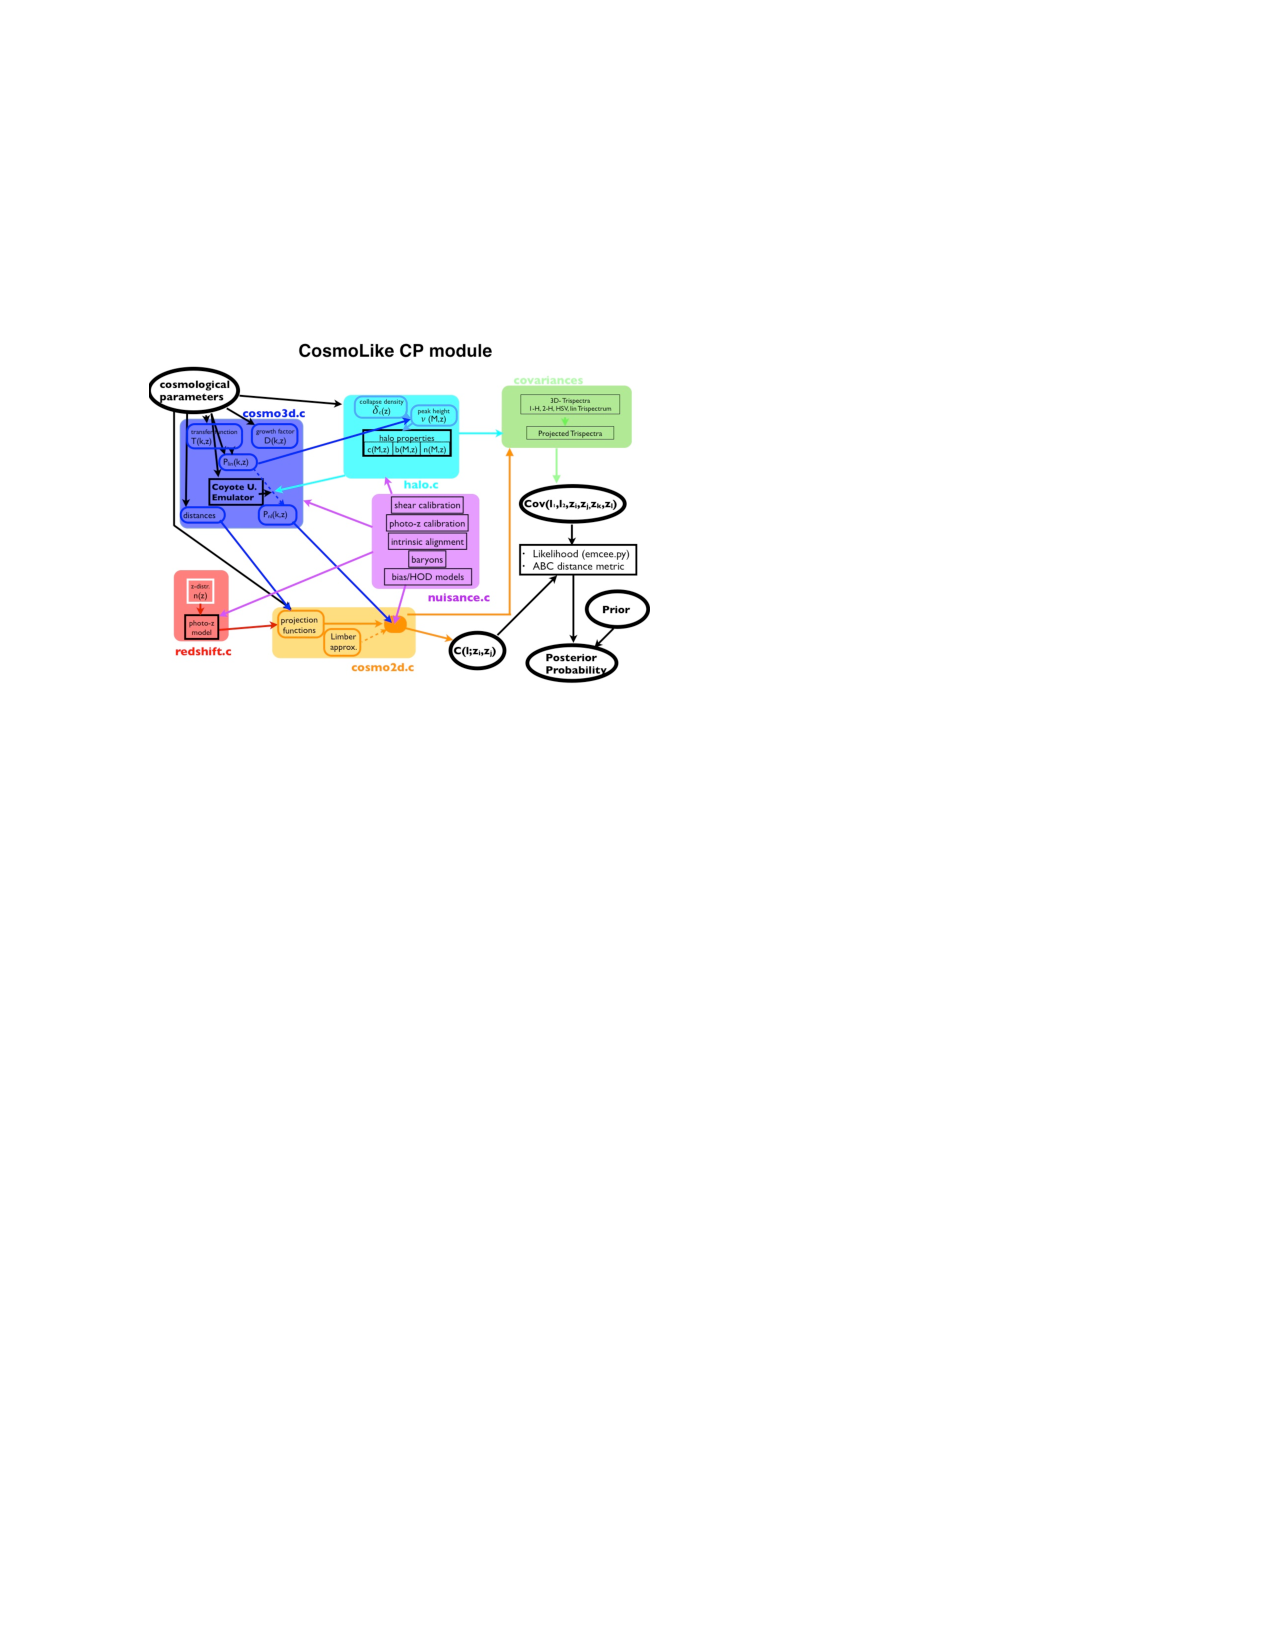
\includegraphics[width=16.0cm]{Plots/forecasts/cosmolike_codestruct}
   \caption{Illustration of a subset of CosmoLike's code structure. Starting from cosmological parameters we give details on how different parts of the code interface and how to finally obtain projected summary statistics for various observables. We note that this particular workflow represents a multi-probe analysis as described in Sect. {\ref{sec:multi-probe}}. For the HLSS survey a subset of the routines is being used.
}
  \label{fi:fcosmolike}
\end{figure*}

CosmoLike is unique in its integrated ansatz of jointly modeling LSS probes and their correlated systematics. It is the only code that computes multi-probe covariances, including the (dominant) higher-order terms of the matter density field. The code has been used to simulate realistic multi-probe likelihood analyses for LSST \citep{Krause2017} that include cosmic shear, galaxy clustering, galaxy-galaxy lensing, cluster number counts and cluster weak lensing. 
The software relies on the massively parallelized computation of fine-tuned look-up tables with a targeted sub-second run-time per point in parameter space. Given the large number of parameters describing systematic effects in future LSS analyses this efficient computation ensures an acceptable turnaround time for the analyses. In particular, it allows for the large number of simulated likelihood analyses that are needed to optimize future surveys. Figure 1 illustrates the CosmoLike combined probes module we plan to use for the proposed analysis. Starting from a cosmological model, this schematic illustrates how projected power spectra for various LSS probes are computed: 
\begin{enumerate}
\item In the first step CosmoLike computes the 3D-density power spectra using one of 3 different methods. The density power spectrum can be modeled using the latest suites of numerical simulations, i.e. the Coyote Universe emulator (Heitmann et al. 2014), or the latest implementation of Halofit (Takahashi et al. 2012), or using a state-of-the-art analytic halo model code \citep{Krause2013}. 
\item Given a survey specific redshift distribution CosmoLike computes projected (tomographic) 2D power spectra for WL, galaxy-galaxy lensing, and galaxy clustering.
\item  For the latter two probes the connection between dark and luminous matter is modeled through either a linear bias model or a sophisticated (but computationally slower) HOD implementation (Krause et al. 2013).
\item The covariance is computed analytically using perturbation theory to include the higher-order moments of the density field, including the Halo Sample Variance contribution that dominates the statistical error budget. This covariance takes all cross-correlations between the different probes into account. 
%\item CosmoLike has various systematics modeling capabilities, in particular it can account for baryonic effects, intrinsic alignment, shear calibration and photo-z uncertainties \citep{Eifler2015, Krause2016, Krause2017}. 
\item If one chooses to use two-point correlation functions instead of power spectra CosmoLike offers an extremely fast Fourier transformation using a Hankel transform. As a default the code is connected to a parallel MCMC sampling technique \citep{Goodman2010}, implemented through the emcee python package \citep{Foreman-Mackey2013}.

\end{enumerate}

   
\subsection{HLSS Forecasts}
We have carried out a trade study of area versus depth for the HLSS only, starting from a baseline survey of 2227 deg2 and a wavelength range of 1.05-1.85 microns. We consider two alternative scenarios, i.e. a survey twice as wide and shallower and a survey half as wide but correspondingly deeper.  

The galaxy redshift distributions were computed using the WFIRST Exposure Time Calculator ETC v14. The H-alpha forecasts are based on the average of the 3 models in Pozzetti et al. (2016), and the [O III] forecasts are based on the Mehta et al. (2015) luminosity function. The resulting redshift distributions are visualized in Fig. 1.
We extend the CosmoLike framework (Eifler et al 2014, Krause\&Eifler 2017) to compute the constraining power of all scenarios on cosmic acceleration, closely following Wang et al (2013). We run 500,000 step MCMC simulated likelihood analysis in a 23 dimensional parameter space. We simultaneously vary 7 cosmological parameters and 16 ?nuisance? parameters describing uncertainties due to the linear galaxy bias model, the non-linear smearing of the BAO feature, peculiar velocity dispersion, power spectrum shot noise, and redshift errors. We assume priors on cosmological parameters from the current state of the art experiments, i.e. the Planck mission, the Baryon Oscillation Spectroscopic Survey, the Joint Lightcurve Analysis, as described in Aubourg et al (2015). 

The information gain is quantified using the standard Dark Energy Task Force FOM and an extended cosmology FOM, which measures the enclosed volume in the full 7-dimensional cosmological parameter space, not just in the 2 dark energy parameters. We will refer to these FOMs as DE-FOM and Cosmo-FOM. 
Compared to our baseline scenarios we find a decreased DE-FOM of 32\% and a decreased Cosmo-FOM of 45\% for the shallow/large area survey. For the deep/small area survey we find an increased DE-FOM of 5\% and an increased Cosmo-FOM of 2\%. We note that these findings are model and prior dependent and recommend further studies varying these input parameters. We also note that the [O III] numbers are pending a future update in part due to the reduction in the baseline telescope temperature to 260 K.
\begin{figure*}
  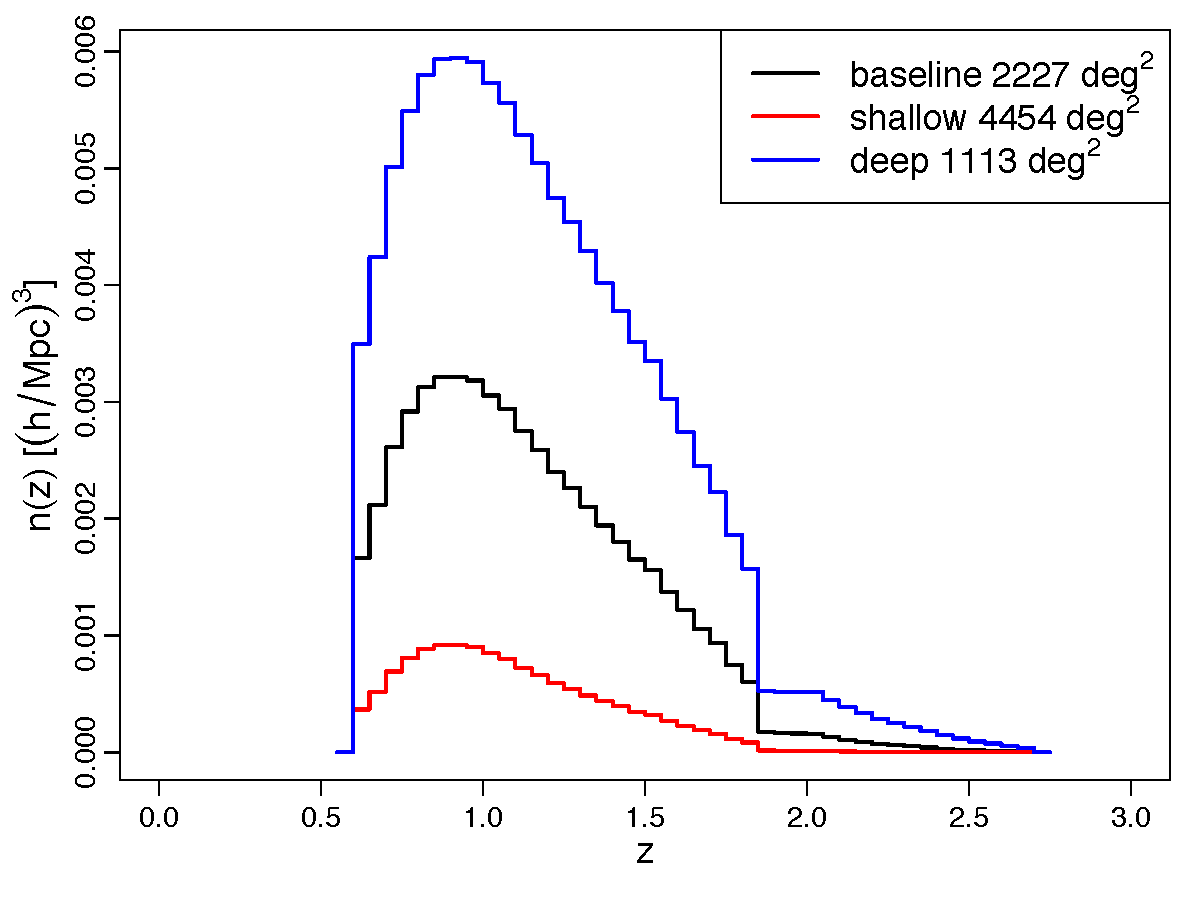
\includegraphics[width=8.0cm]{Plots/forecasts/forecast_1}
  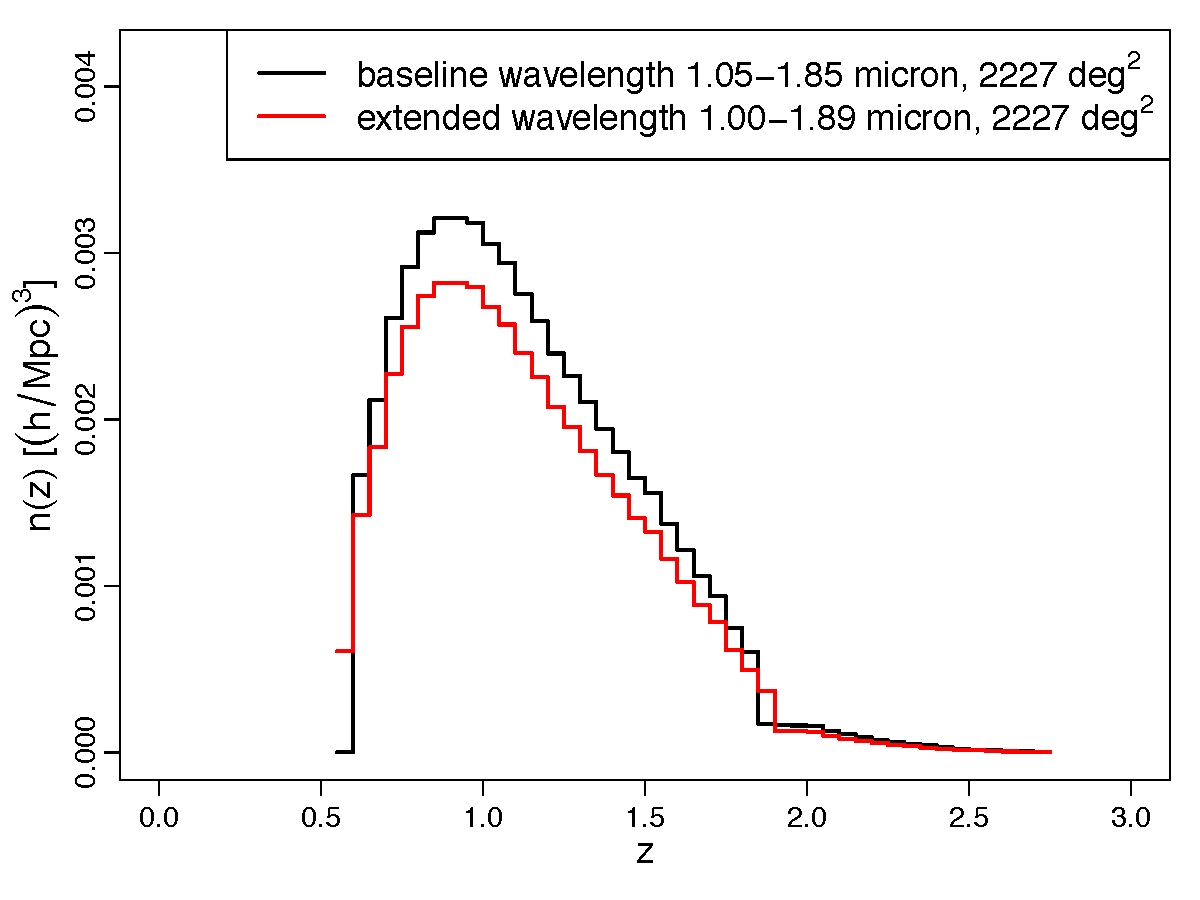
\includegraphics[width=8.0cm]{Plots/forecasts/forecast_2}
   \caption{\textit{left:}Redshift distribution of galaxies of the baseline, the shallow/large area and the deep/small area survey. \textit{right:} Redshift distribution of galaxies of the baseline and extended wavelength survey. 
}
  \label{fi:forecast1}
\end{figure*}

HLSS 3: The redshift range of galaxies surveyed shall encompass 1. ? z ? 2.7 (3 desired, max z TBC depending on telescope temperature trade)


In addition to the trade studies in HLSS 1 we examine the impact of an extended wavelength range on the DE-FOM and the Cosmo-FOM. We follow the same procedure as detailed in the HLSS 1 paragraph extending the wavelength range from 1.05-1.85 microns for the baseline model to 1.00-1.89 for the extended model. The corresponding redshift distributions of the galaxy samples computed from the ETC v1.14 are depicted in Fig. 2. We find a decreased DE-FOM of 2\% and a decreased Cosmo-FOM of 11\% for the extended wavelength survey with respect to our baseline scenario. We iterate that these findings are model and prior dependent and recommend further studies varying these input parameters.

\subsection{HLIS Forecasts}
\label{sec:HLISforecasts}



\begin{figure*}
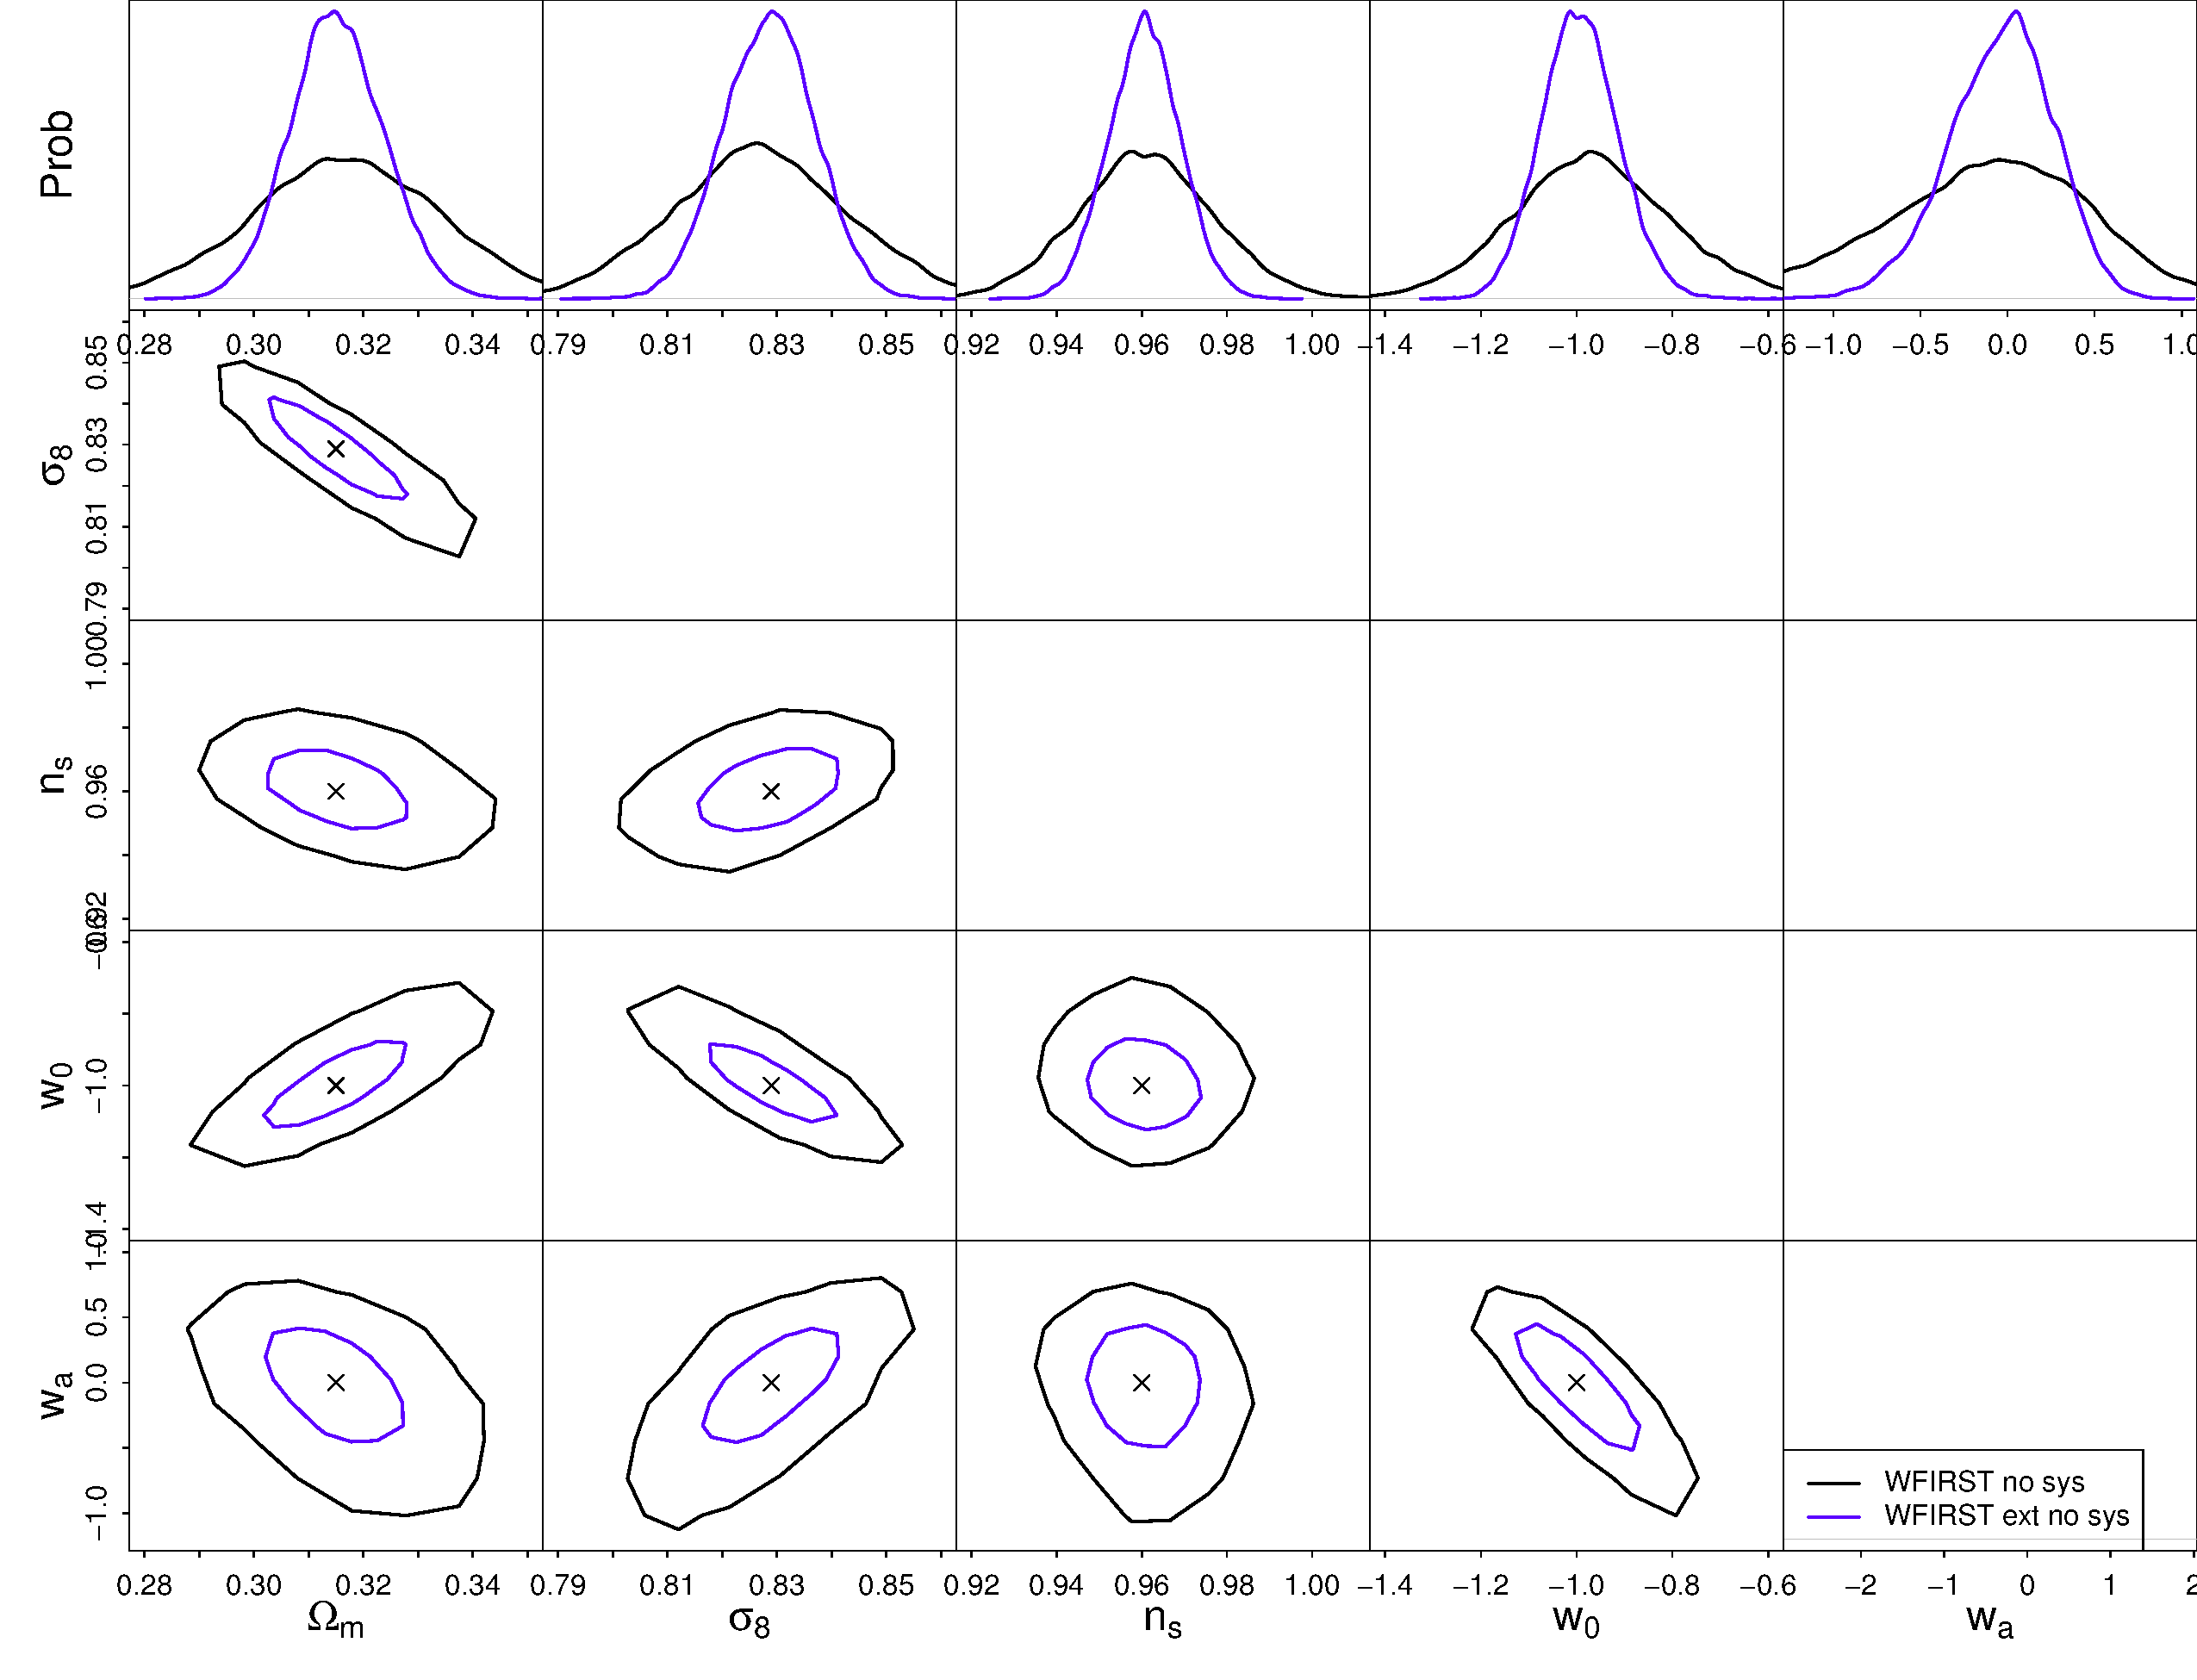
\includegraphics[width=17cm]{Plots/forecasts/WFIRST_no_sys.eps}
\caption{WFIRST forecasts statistical errors only. Extended Mission 10,000 $\mr{deg^2}$ in blue, regular mission 2200 $\mr{deg^2}$ in black}
         \label{fi:lsst1}
\end{figure*}

\begin{figure*}
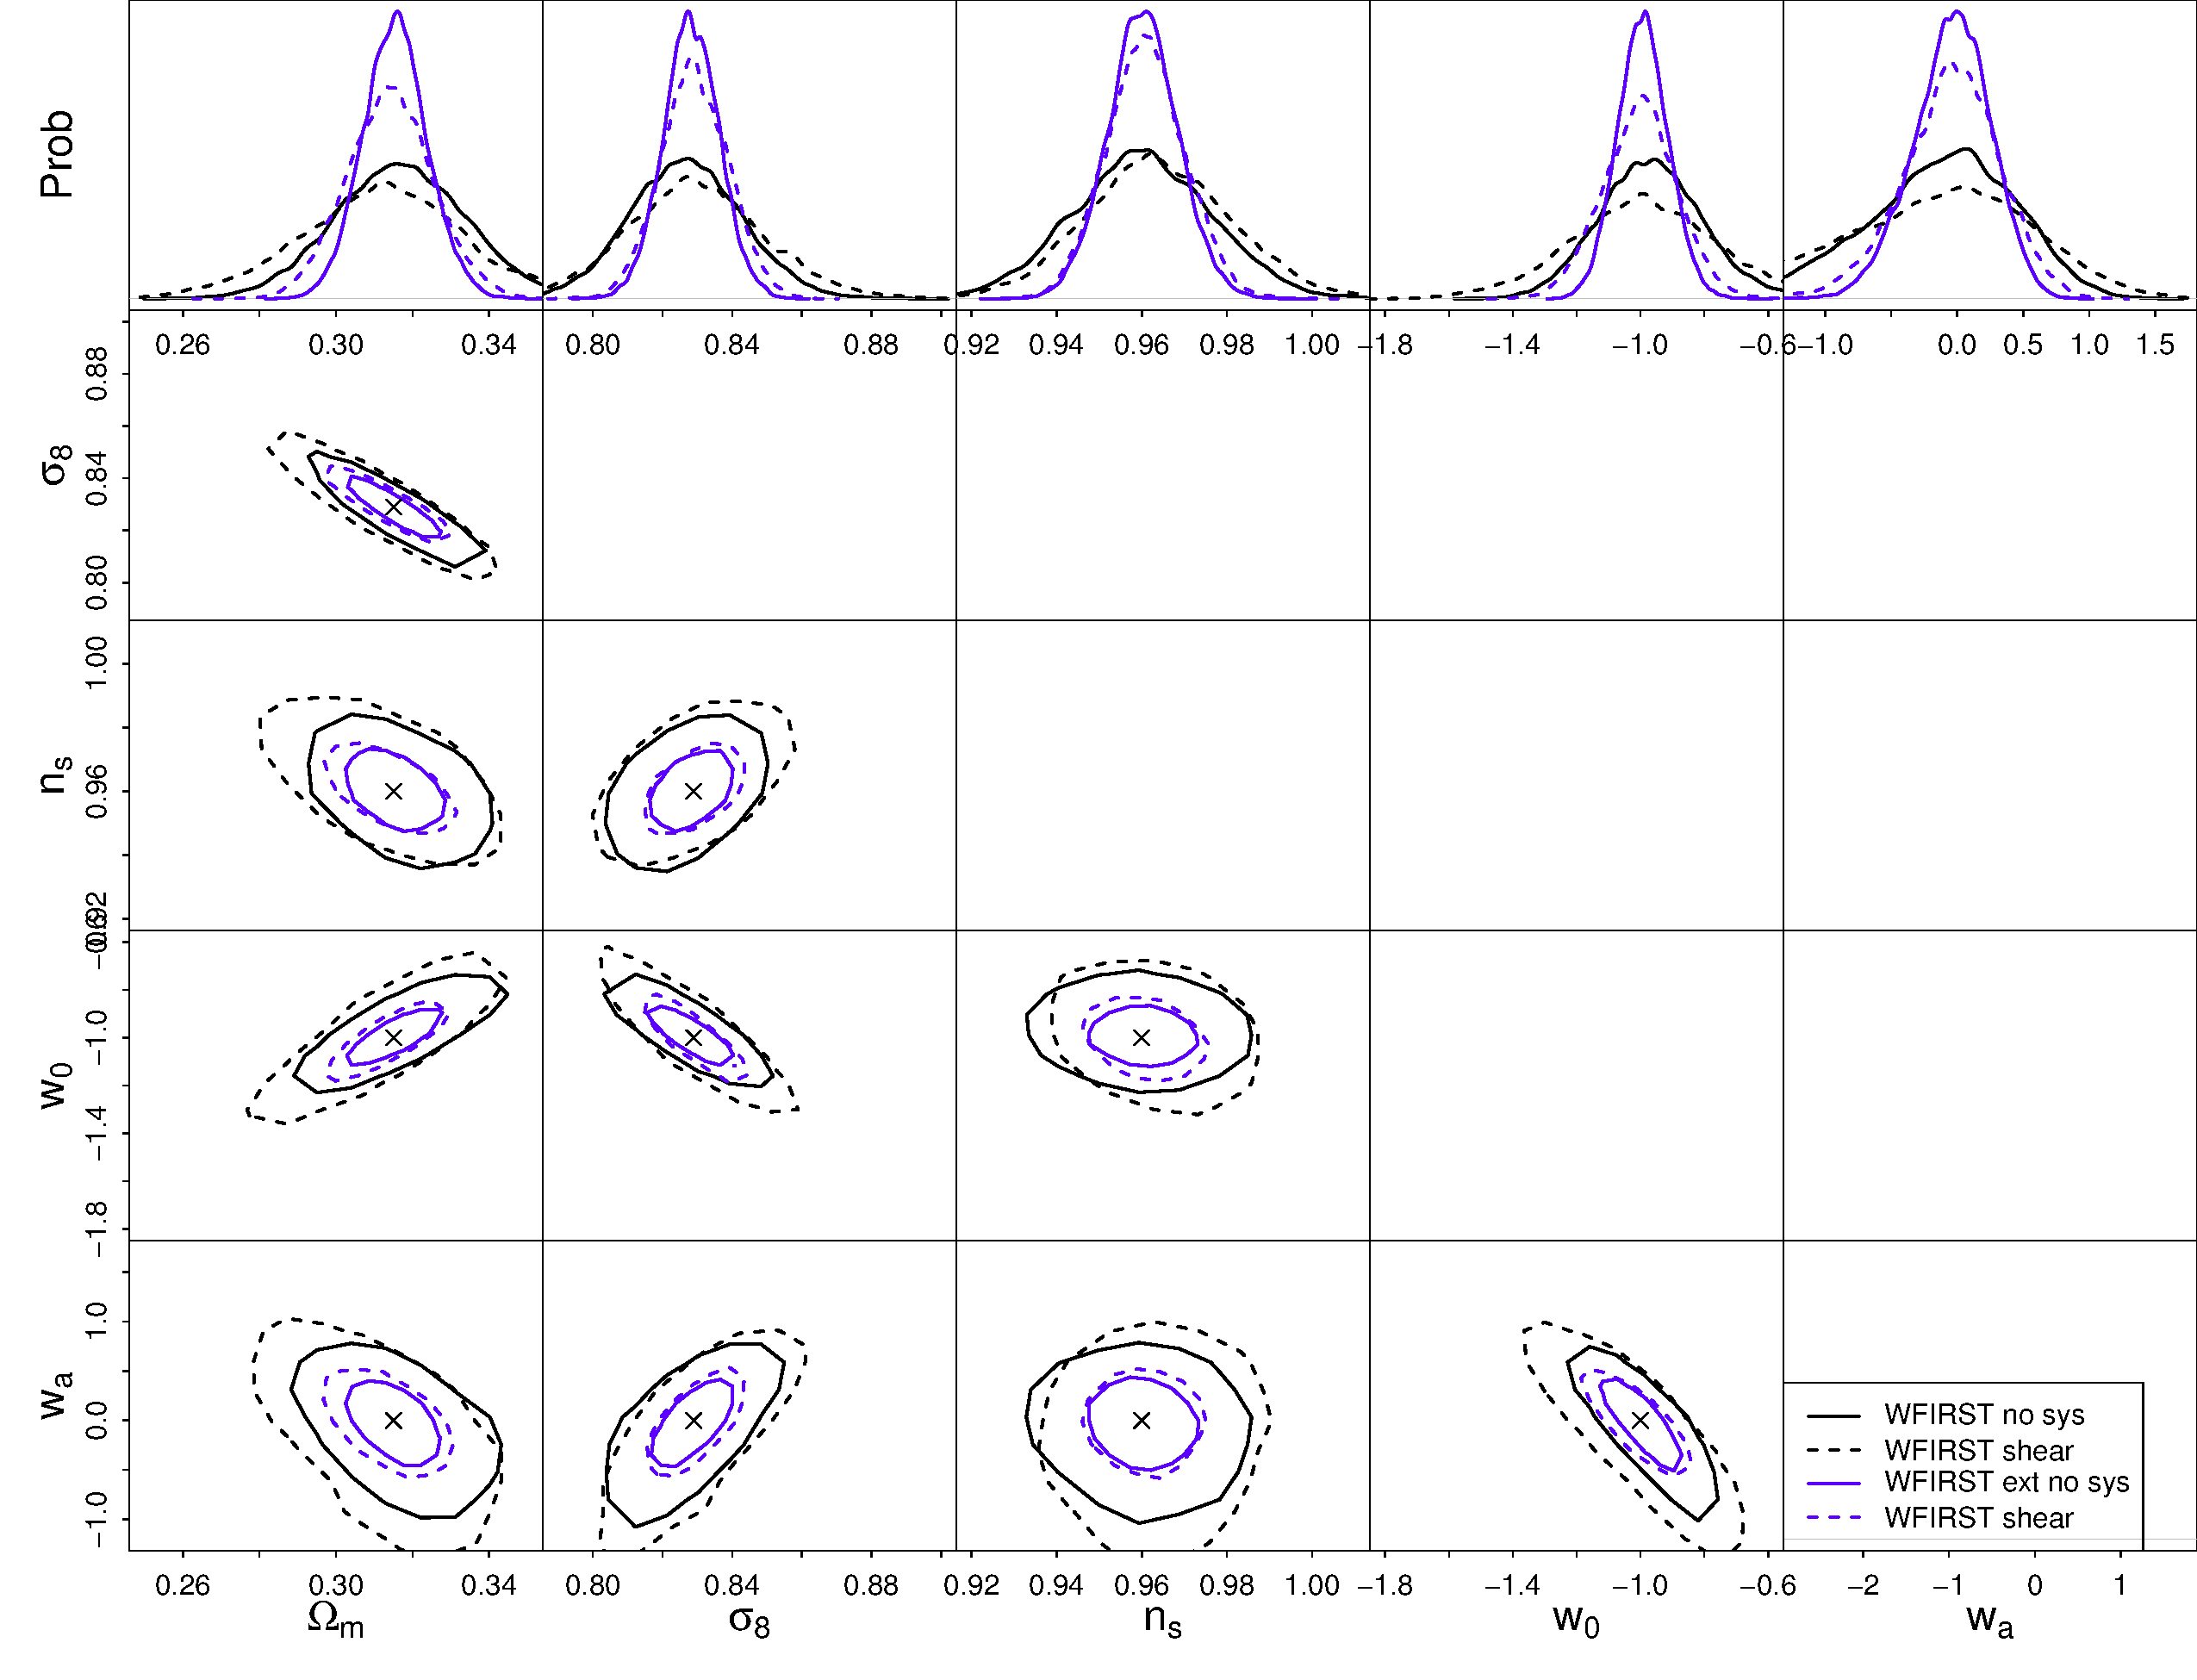
\includegraphics[width=17cm]{Plots/forecasts/WFIRST_shear.eps}
\caption{WFIRST forecasts statistical errors (solid) compared to errors when including uncertainties from multiplicative shear calibration errors (dashed). Shear calibration uncertainties are modeled as a Gaussian with $\sigma=0.005$. Extended Mission 10,000 $\mr{deg^2}$ in blue, regular mission $2200 \mr{deg^2}$ in black}
         \label{fi:lsst1}
\end{figure*}

\begin{figure*}
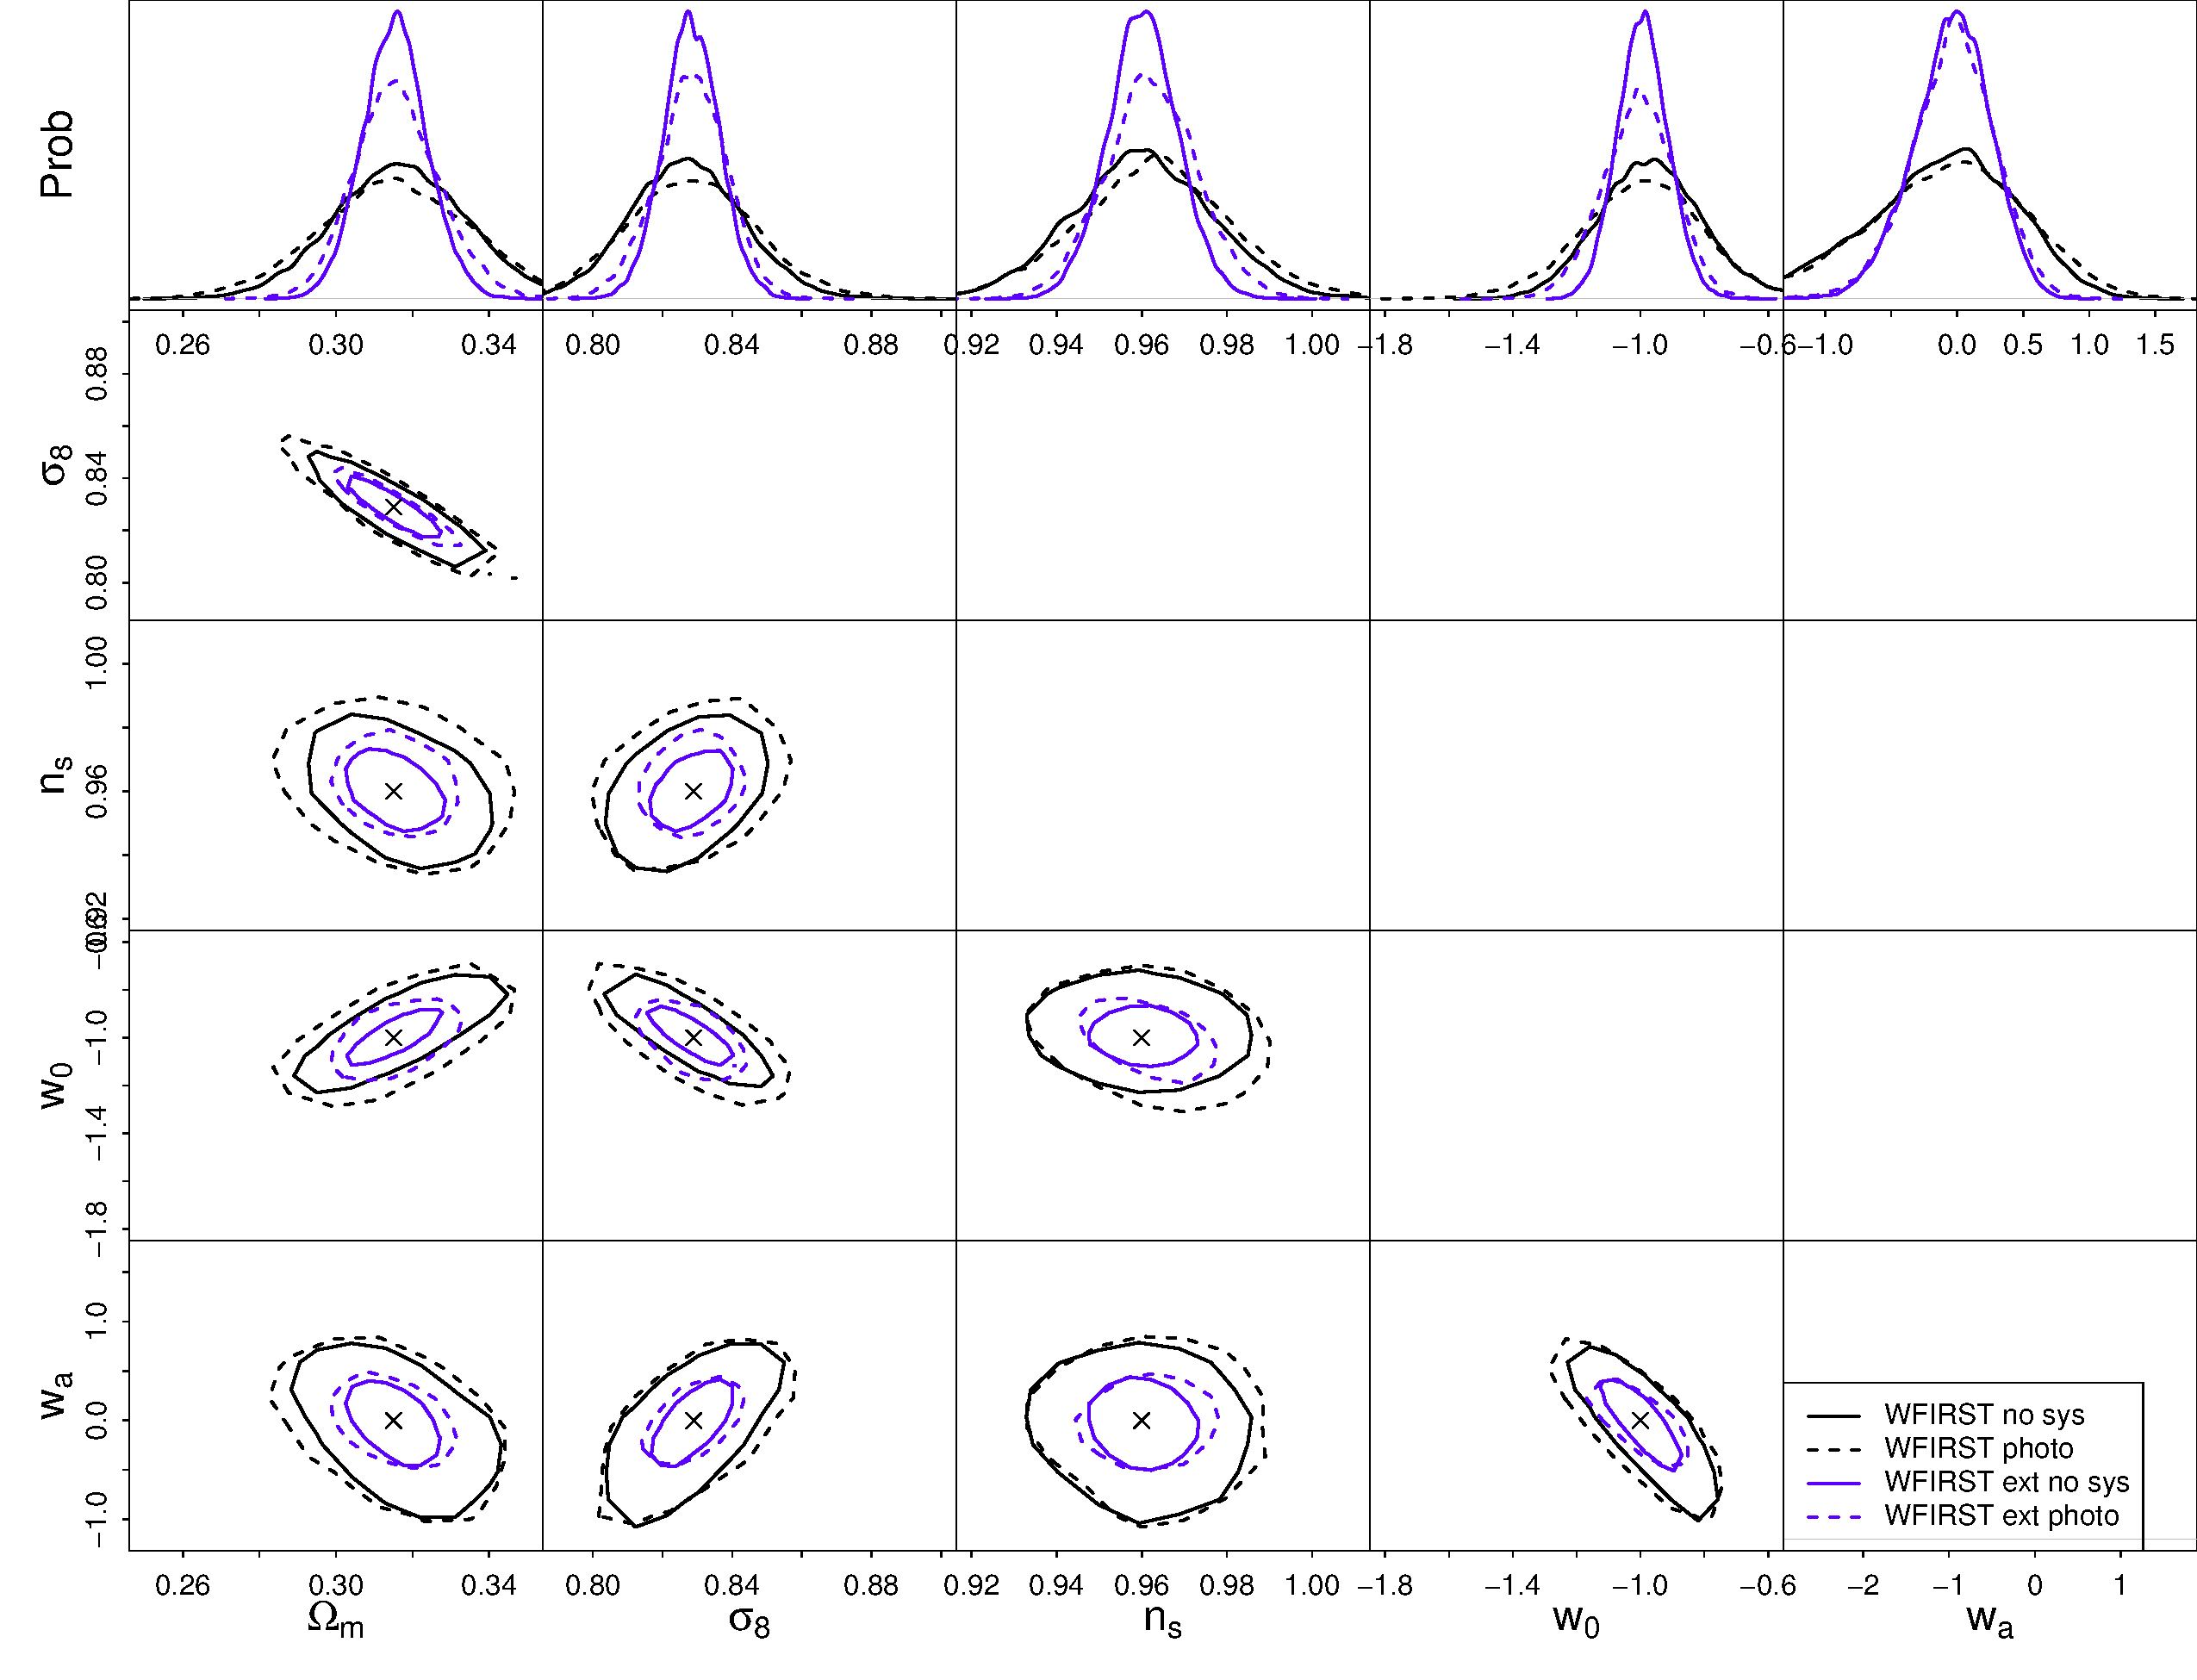
\includegraphics[width=17cm]{Plots/forecasts/WFIRST_photo.eps}
\caption{WFIRST contours when accounting for photo-z uncertainties. We model these as Gaussian photo-z errors with a bias around mean zero and $\sigma=0.05$. These 2 parameters (bias and $sigma$) again have Gaussian priors, i.e. $\Delta \mr{bias}=0.005$ and $\Delta \sigma=0.006$.}
         \label{fi:lsst1}
\end{figure*}

\begin{figure*}
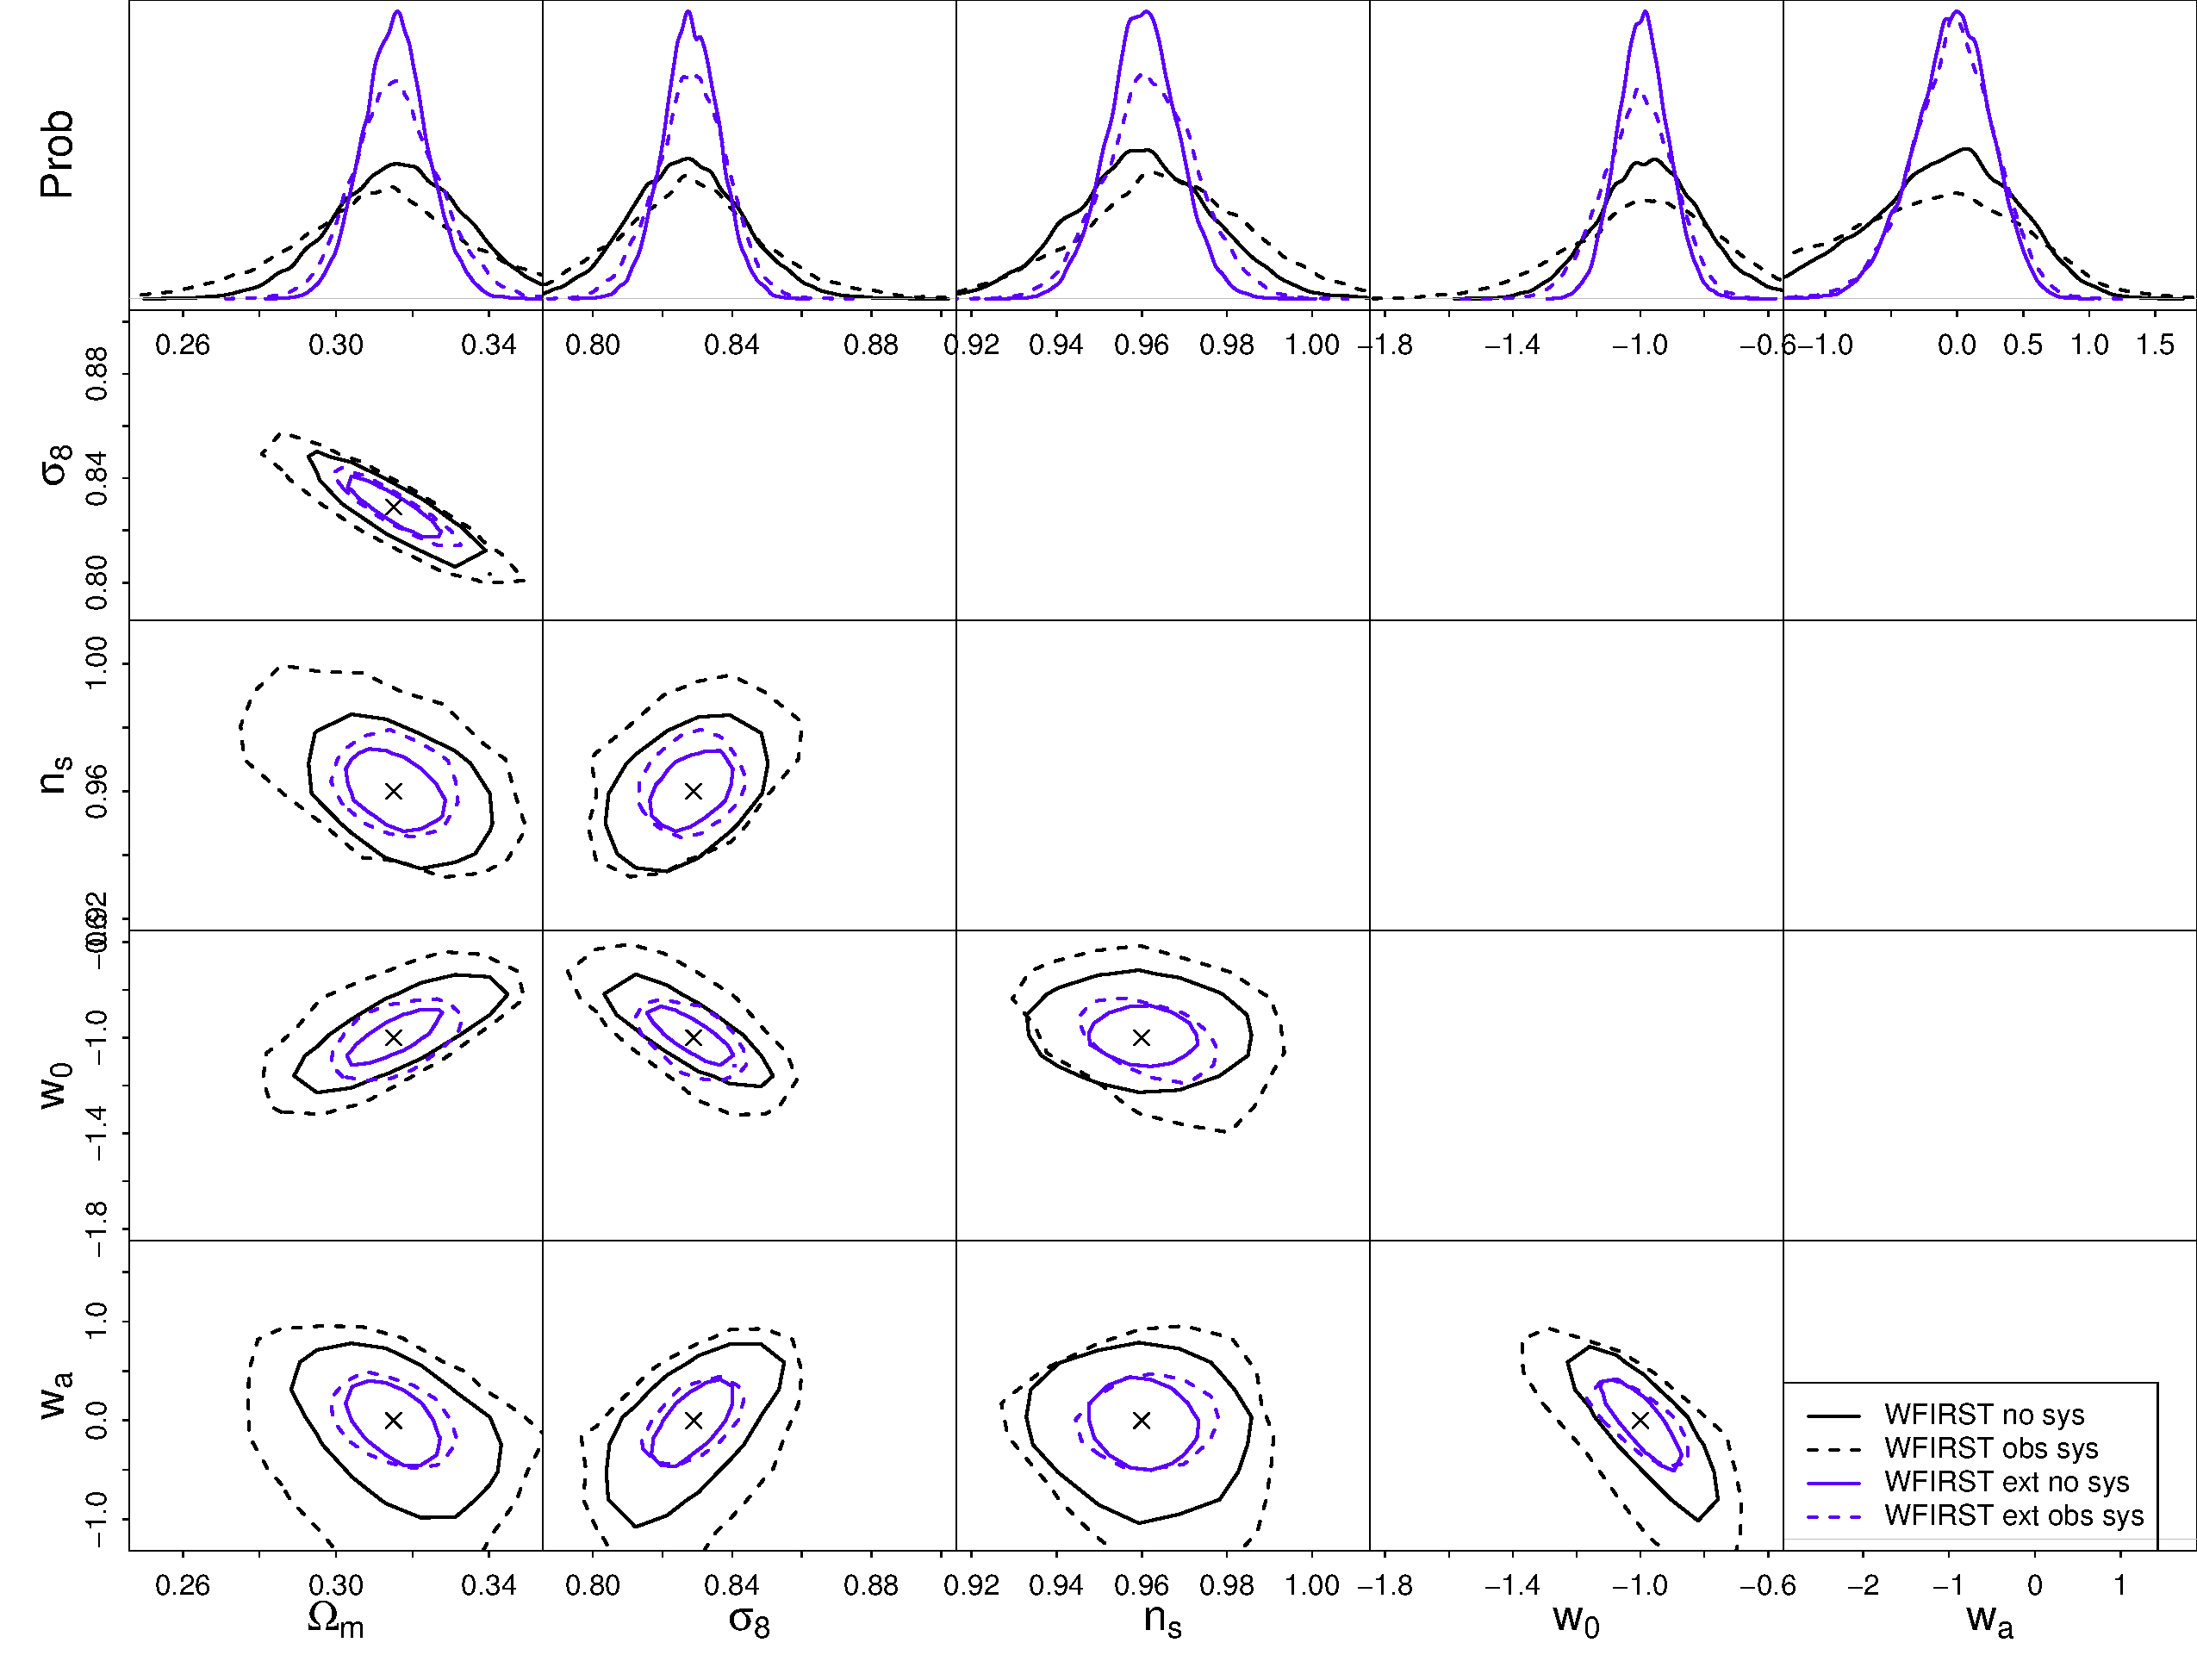
\includegraphics[width=17cm]{Plots/forecasts/WFIRST_obs_sys.eps}
\caption{Broadening of WFIRST error bars accounting for shear calibration and photo-z errors}
         \label{fi:lsst1}
\end{figure*}

\begin{figure*}
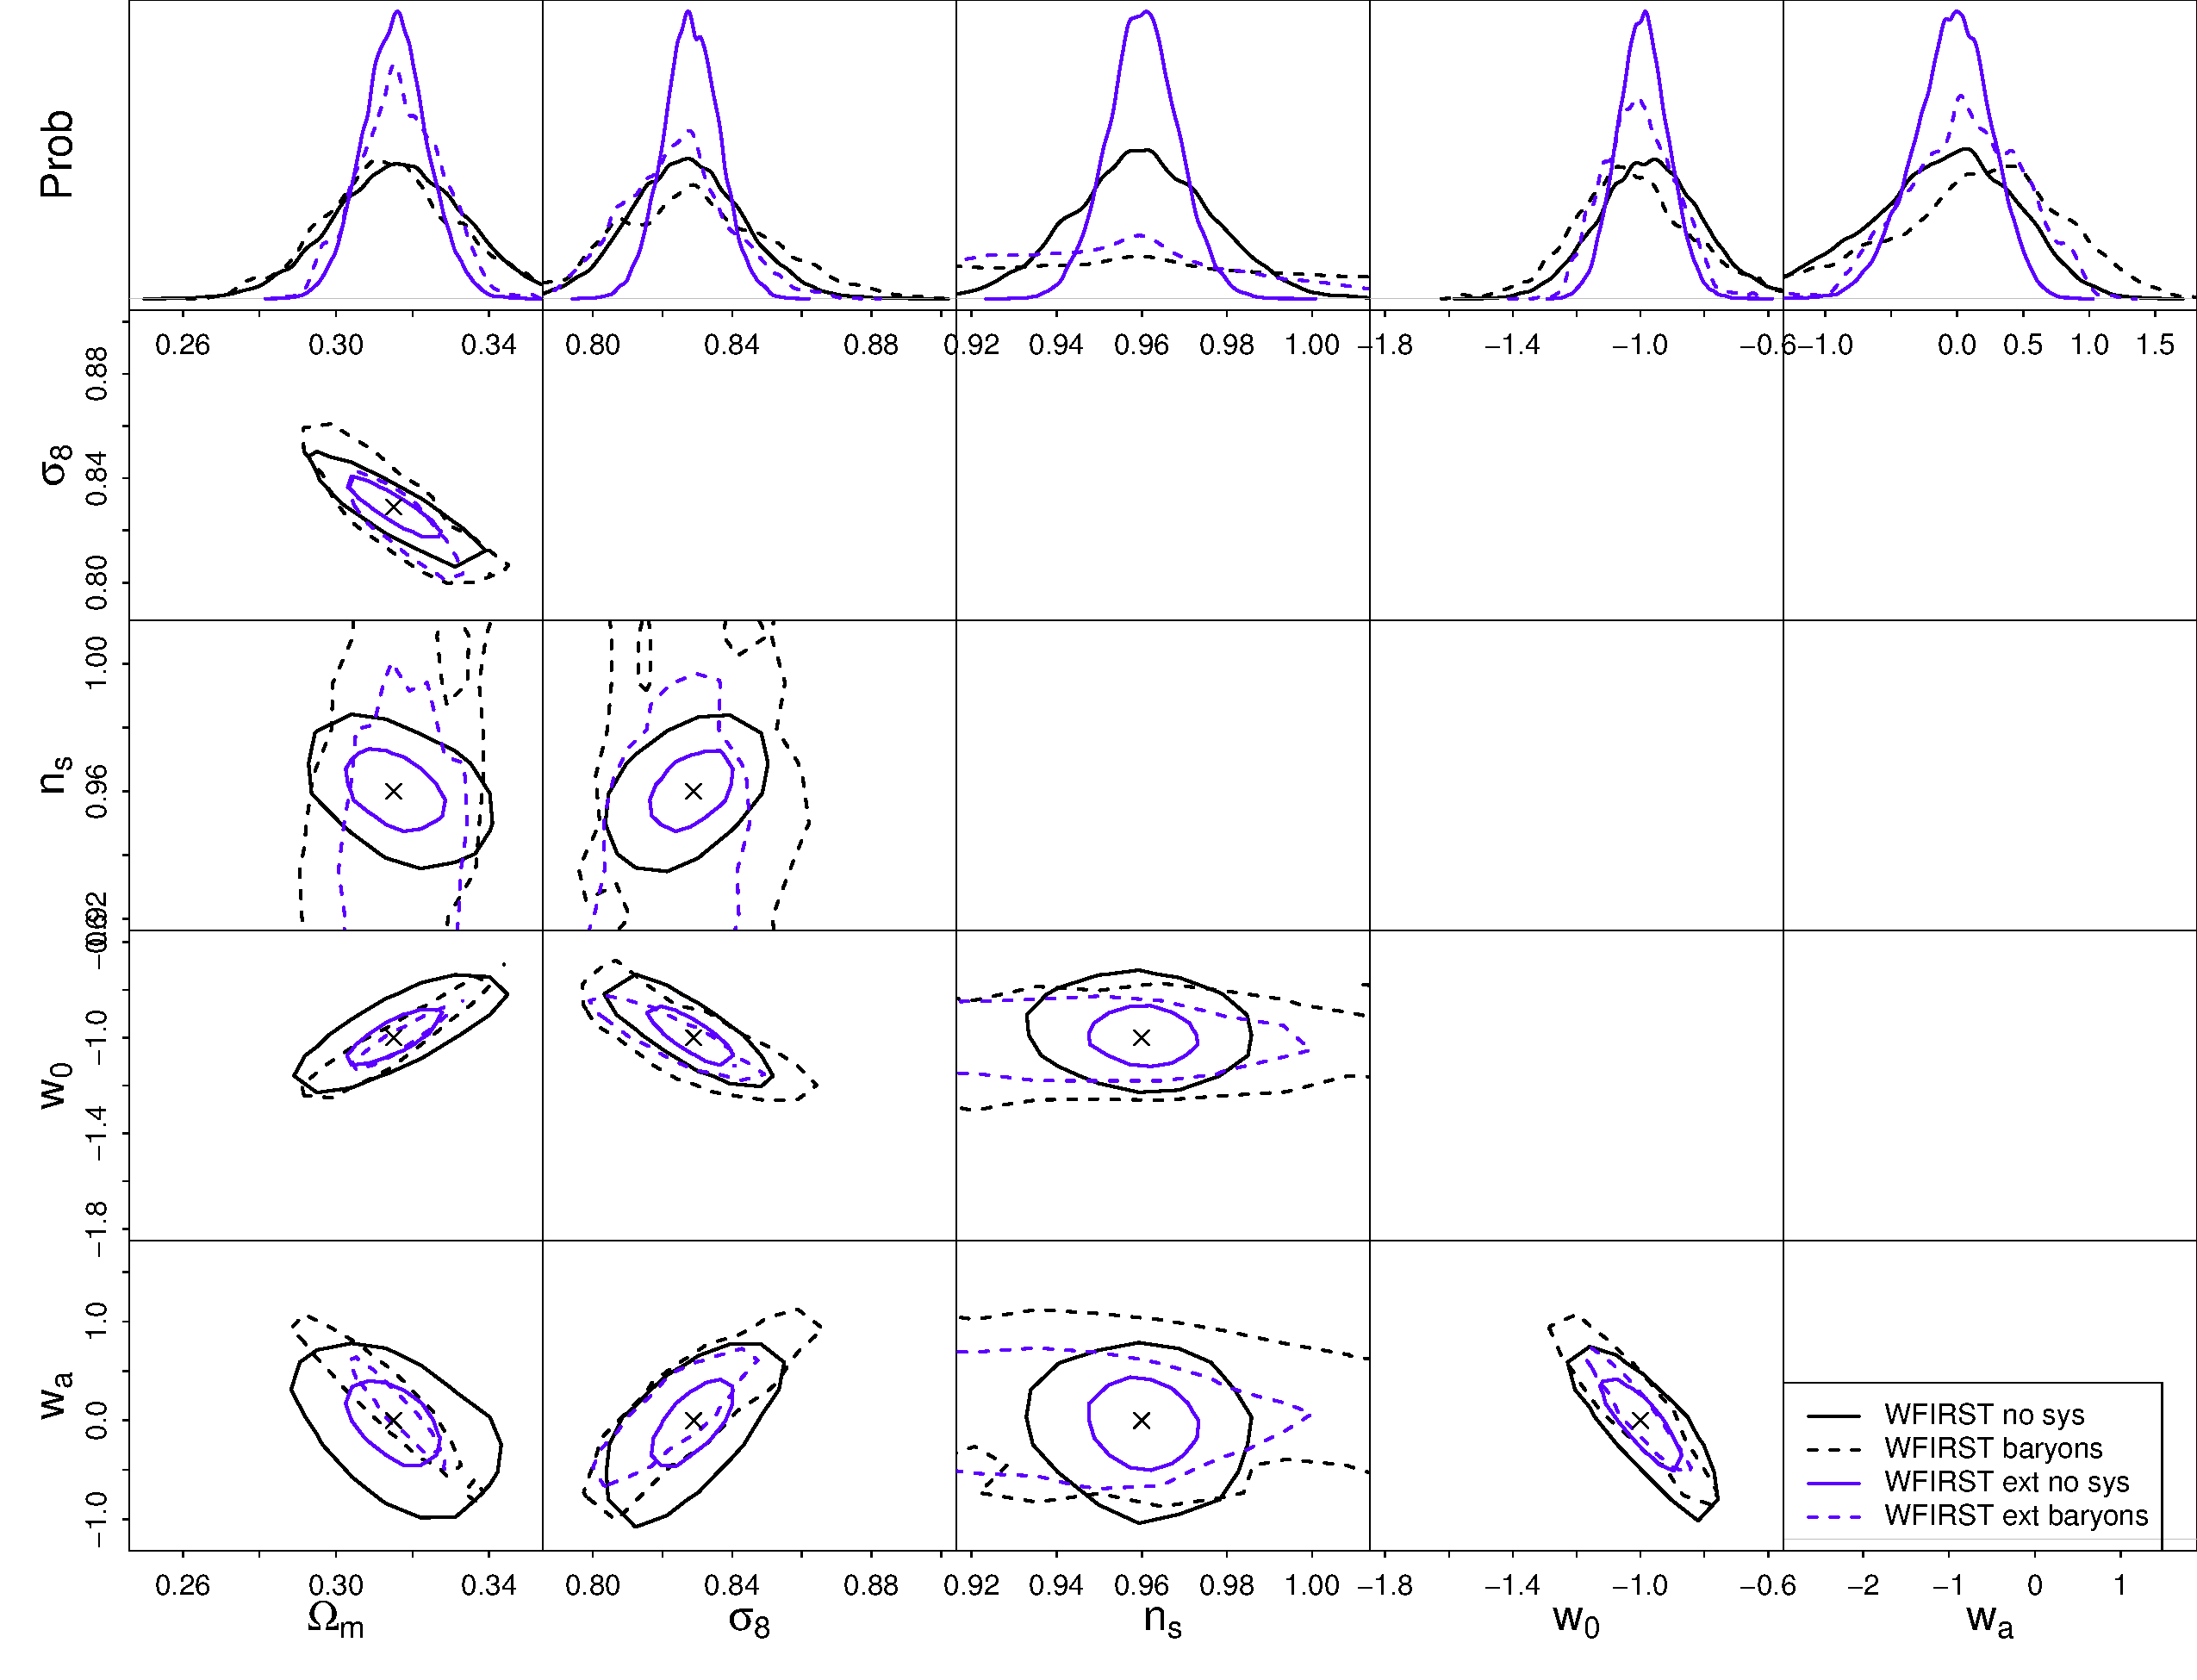
\includegraphics[width=17cm]{Plots/forecasts/WFIRST_baryons.eps}
\caption{Broadening of WFIRST error bars when accounting for baryons.}
         \label{fi:lsst1}
\end{figure*}

\begin{figure*}
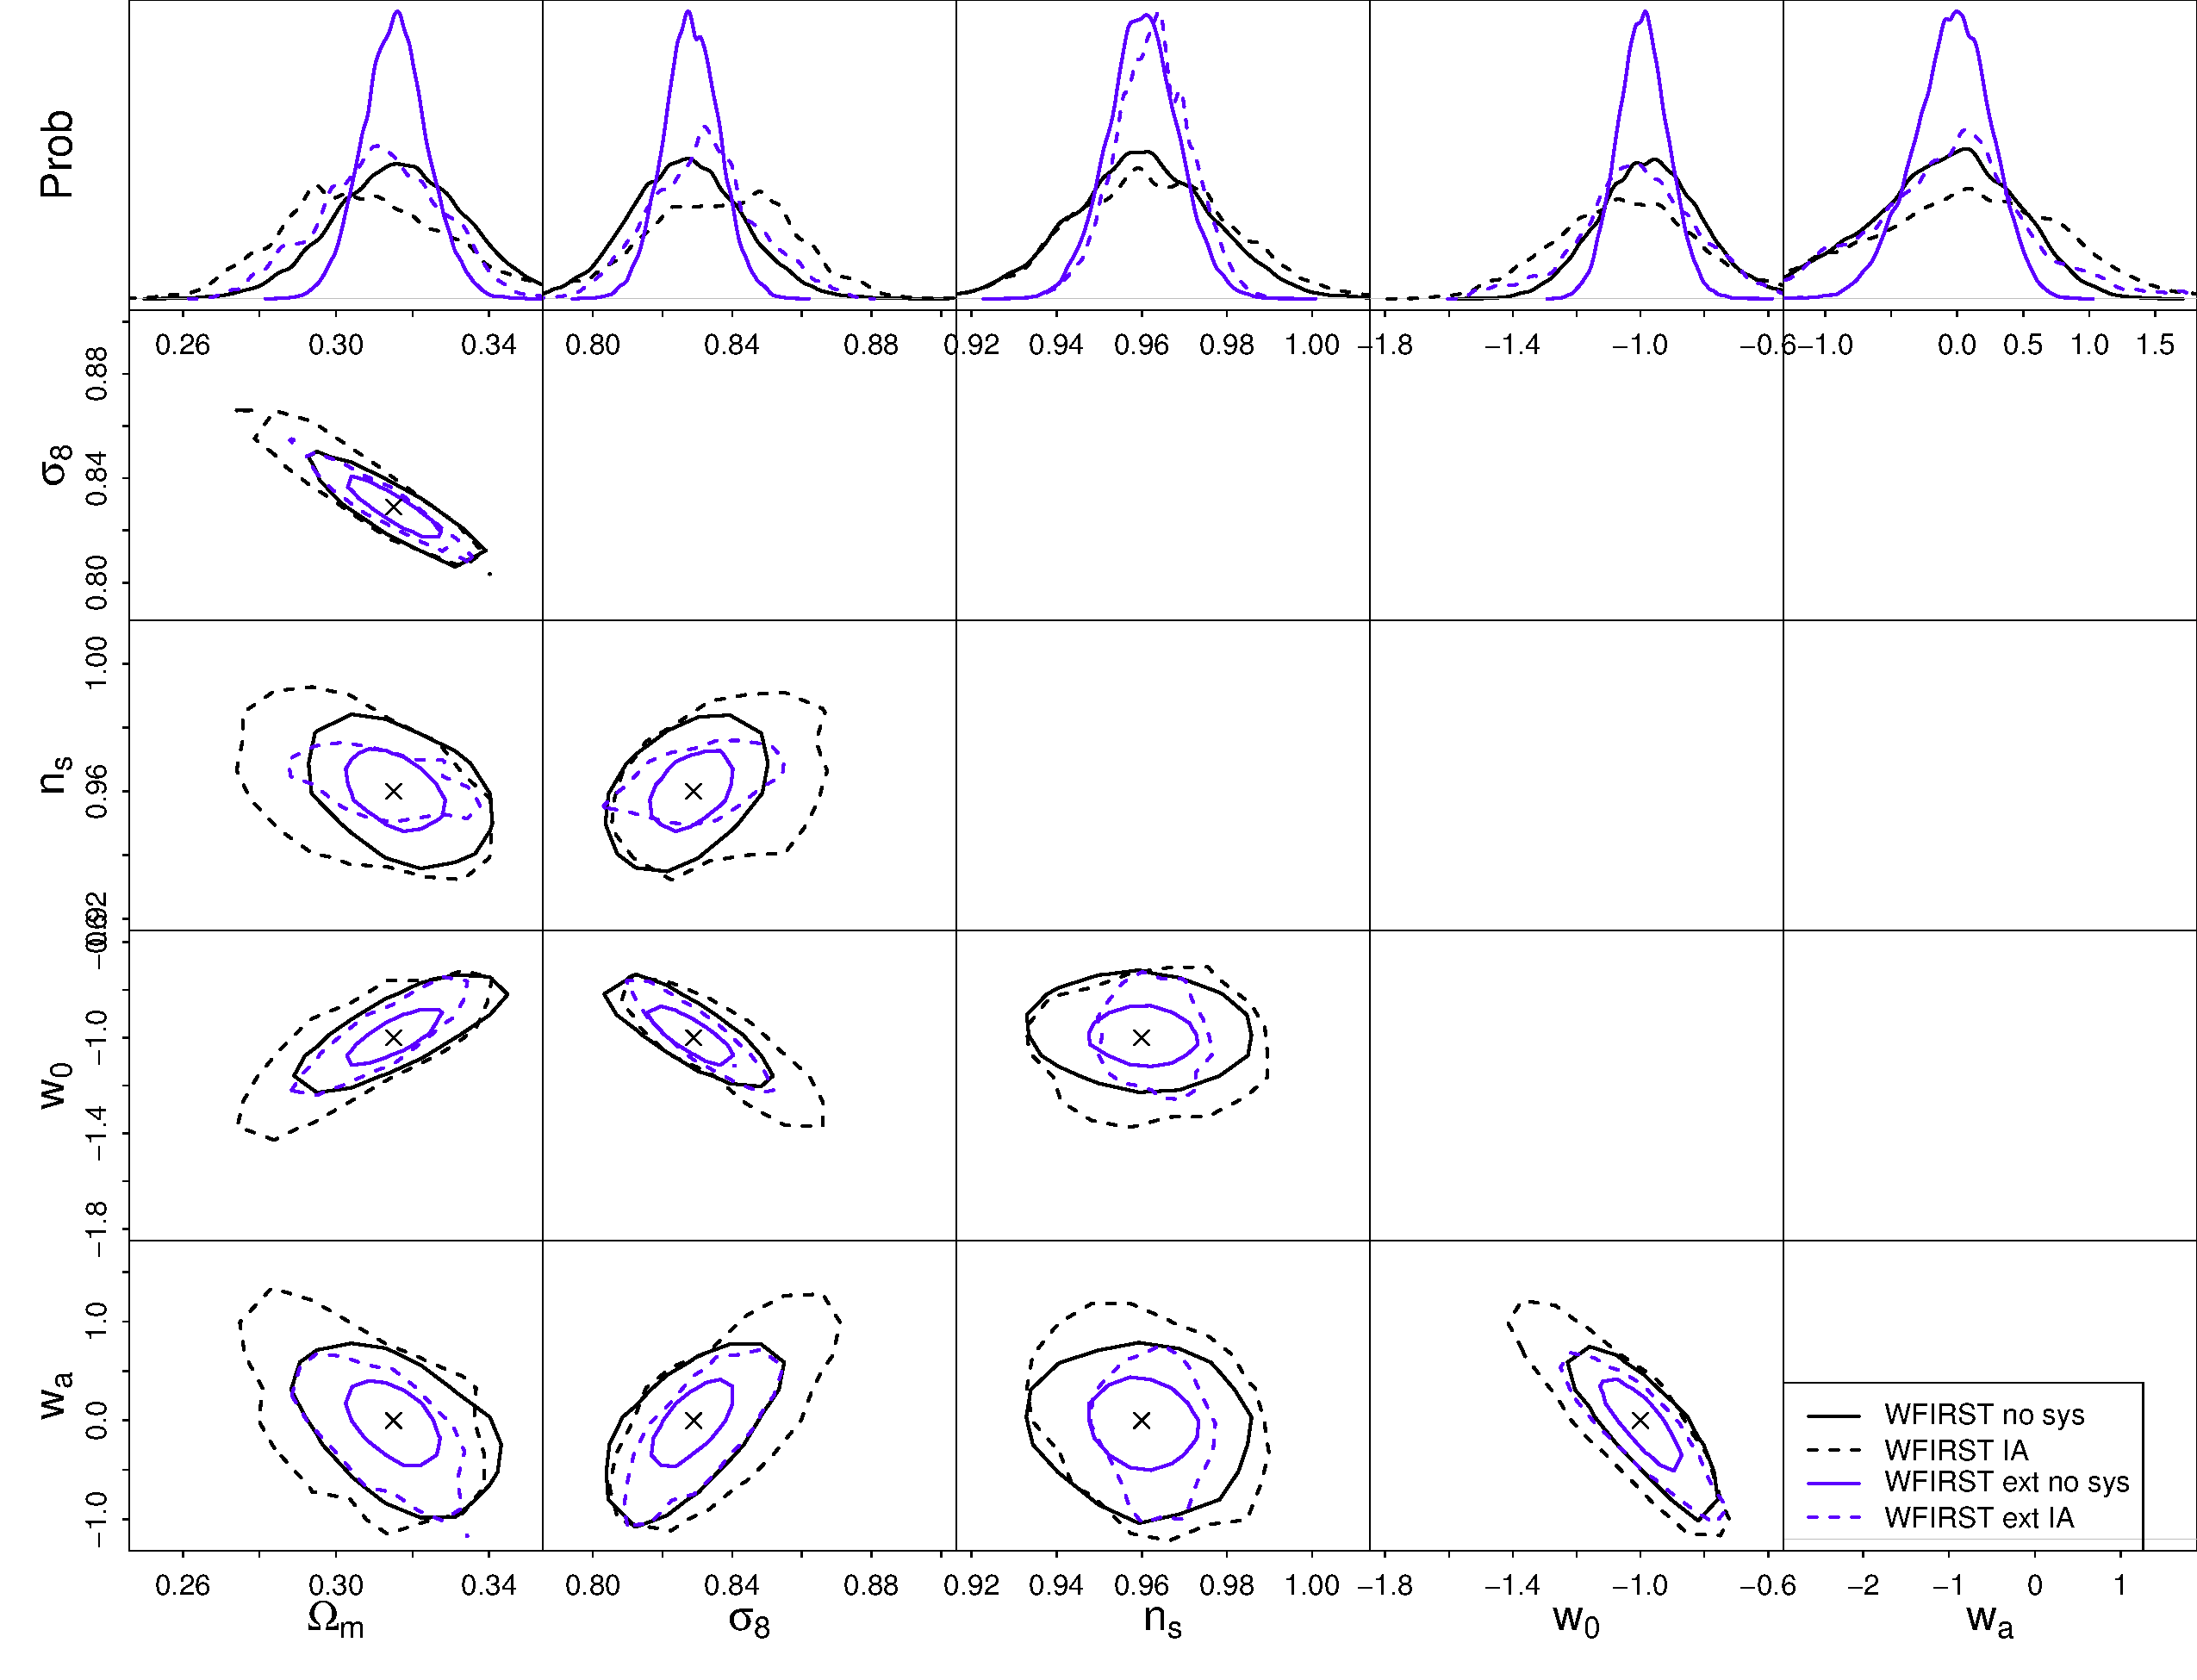
\includegraphics[width=17cm]{Plots/forecasts/WFIRST_ia.eps}
\caption{Broadening of WFIRST error bars when accounting for intrinsic alignment.}
         \label{fi:lsst1}
\end{figure*}



\begin{figure*}
\includegraphics[width=17cm]{Plots/forecasts/WFIRST_bary_impact.eps}
\caption{LSST IA marg}
         \label{fi:lsst1}
\end{figure*}

\begin{figure*}
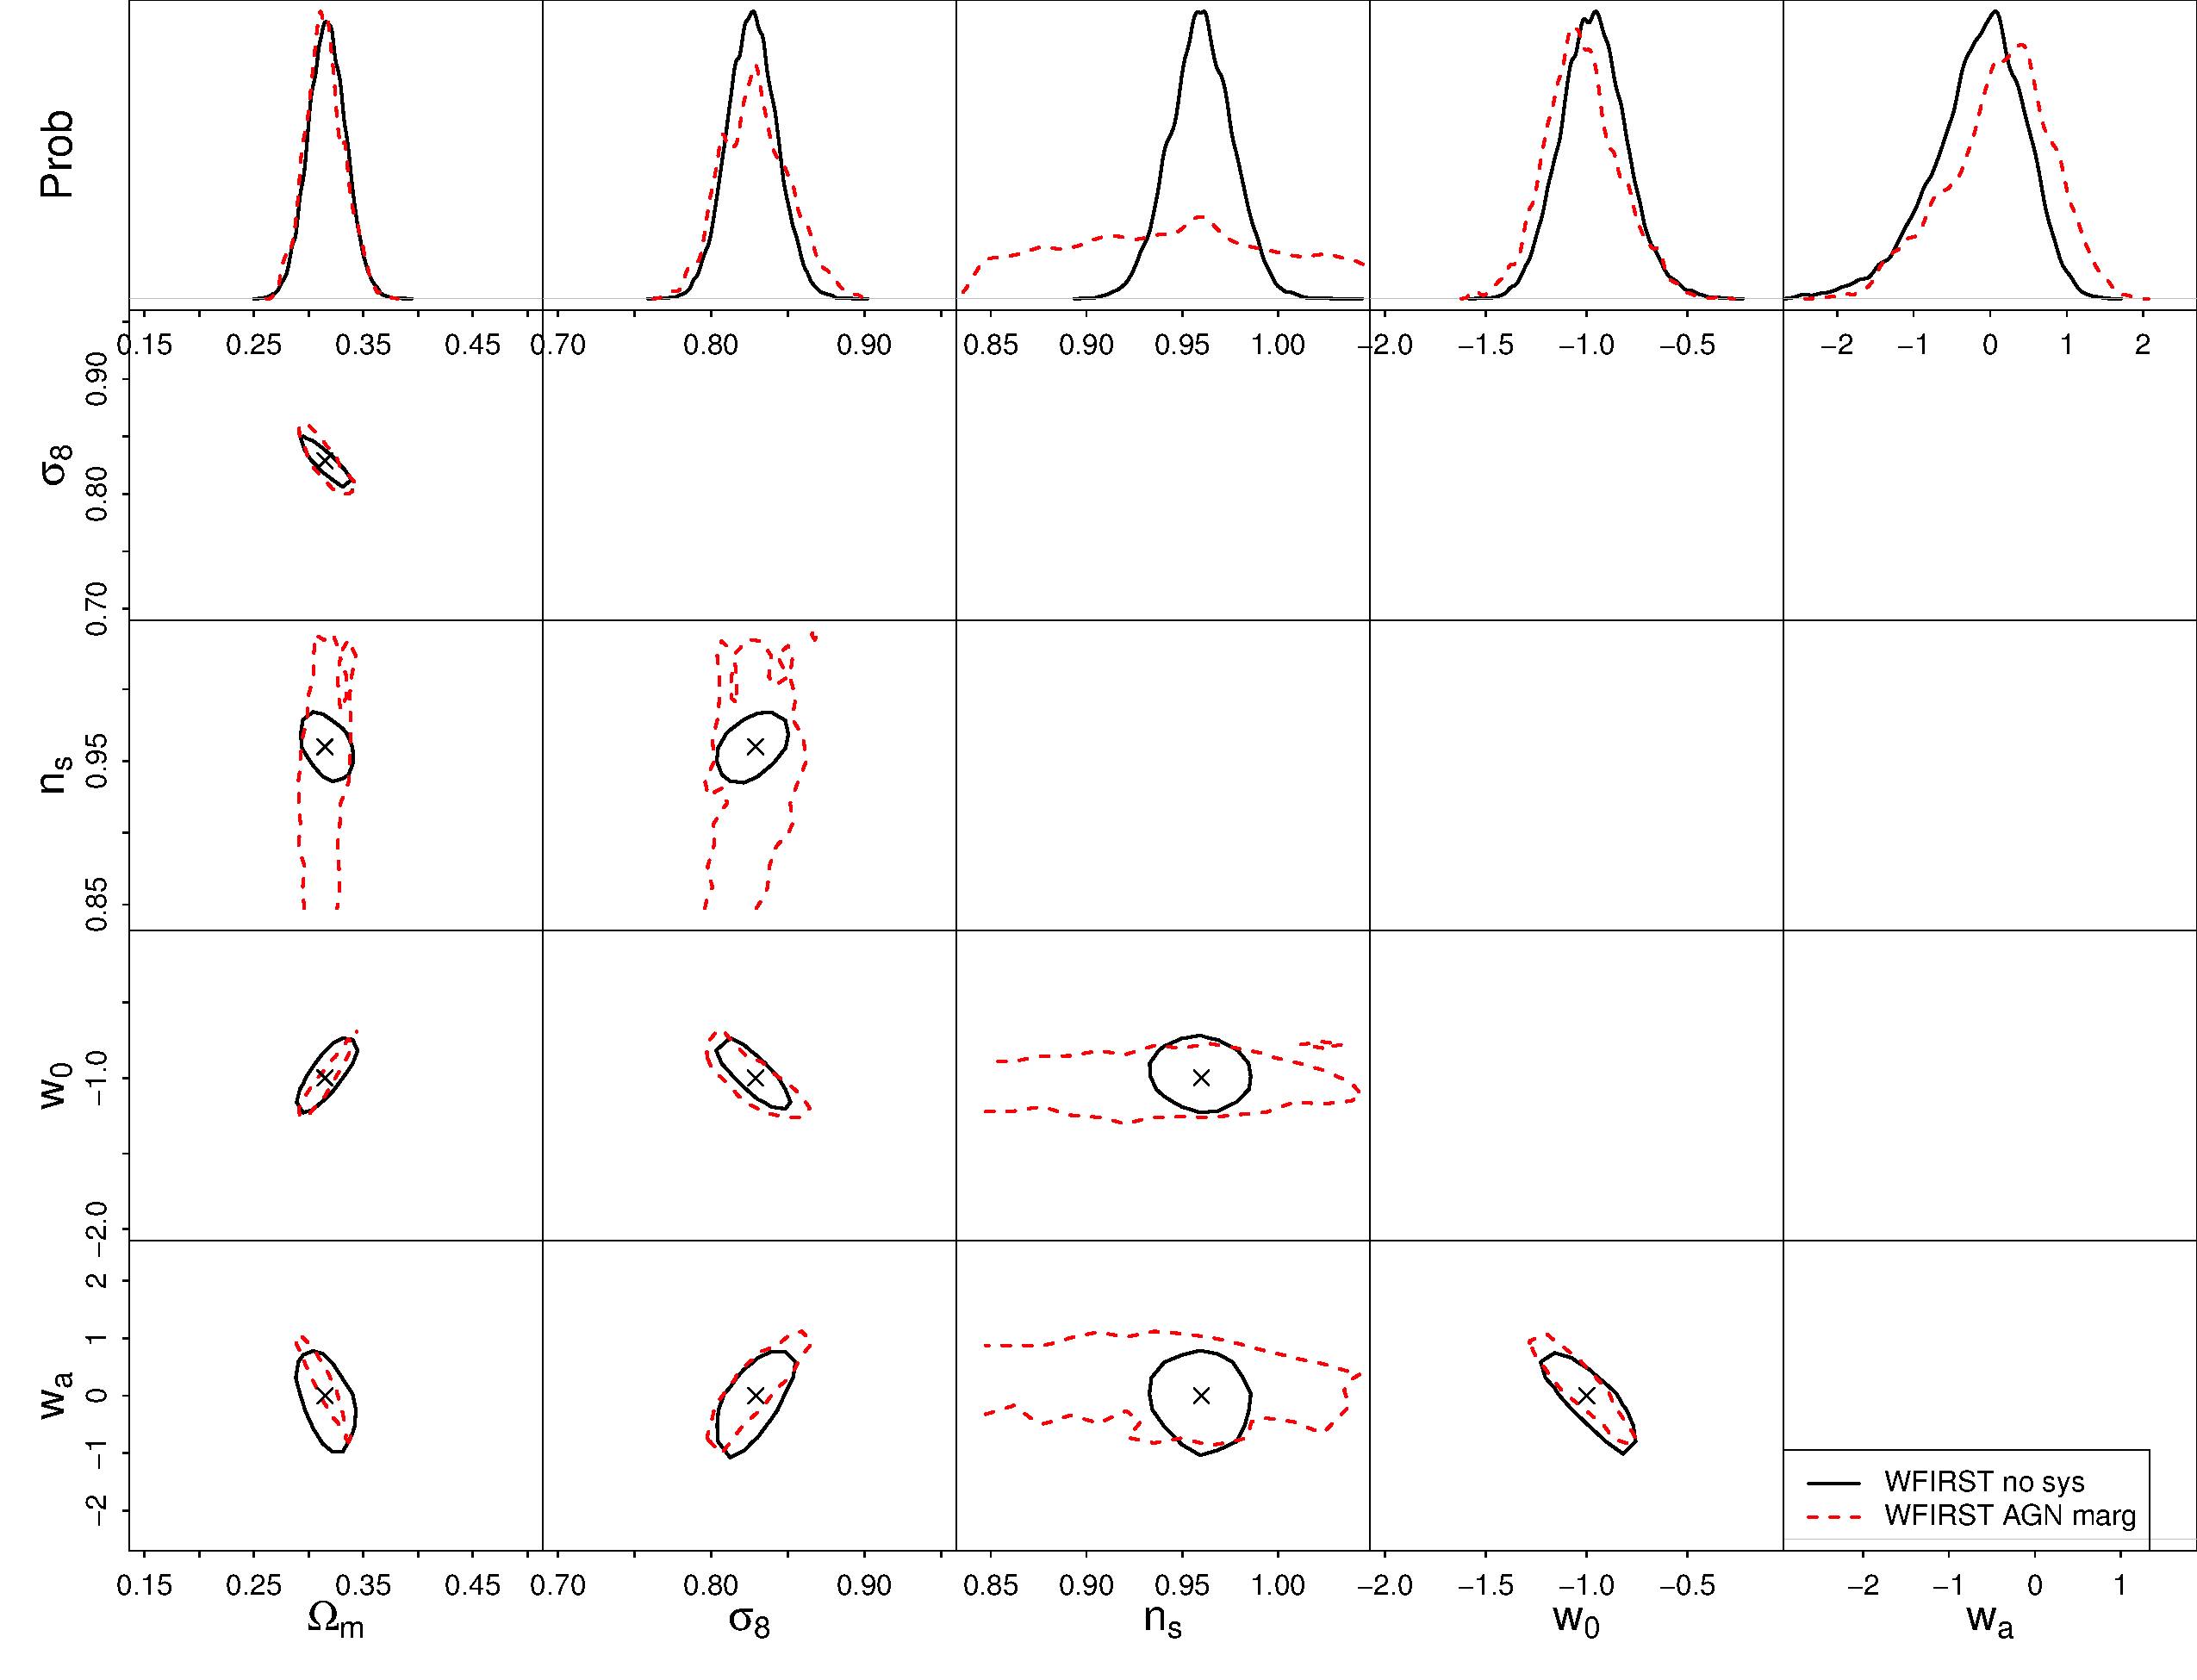
\includegraphics[width=17cm]{Plots/forecasts/WFIRST_bary_miti.eps}
\caption{LSST IA marg}
         \label{fi:lsst1}
\end{figure*}


\subsection{Expanding the Science Case - Multi-Probe Forecasts}
\label{sec:multi-probe}

\begin{figure*}
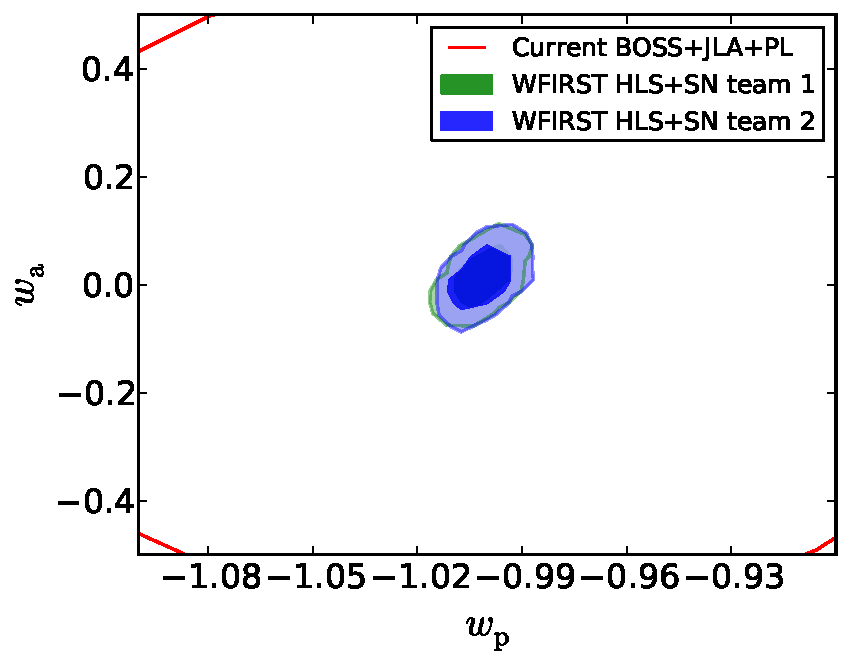
\includegraphics[width=8cm]{Plots/forecasts/WFIRST_2SNteams_zoom.pdf}
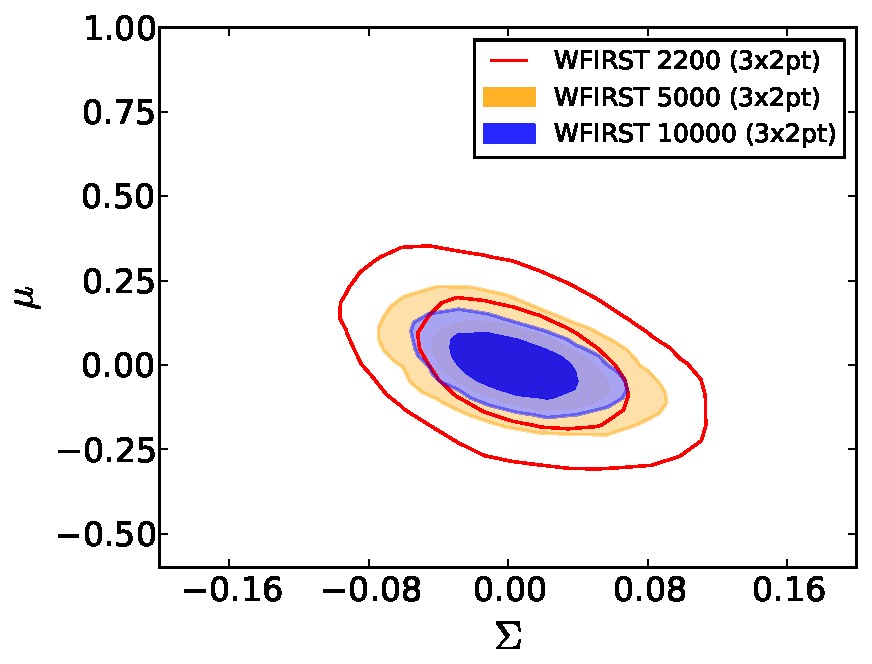
\includegraphics[width=8cm]{Plots/forecasts/WFIRST_extended_MG.pdf}
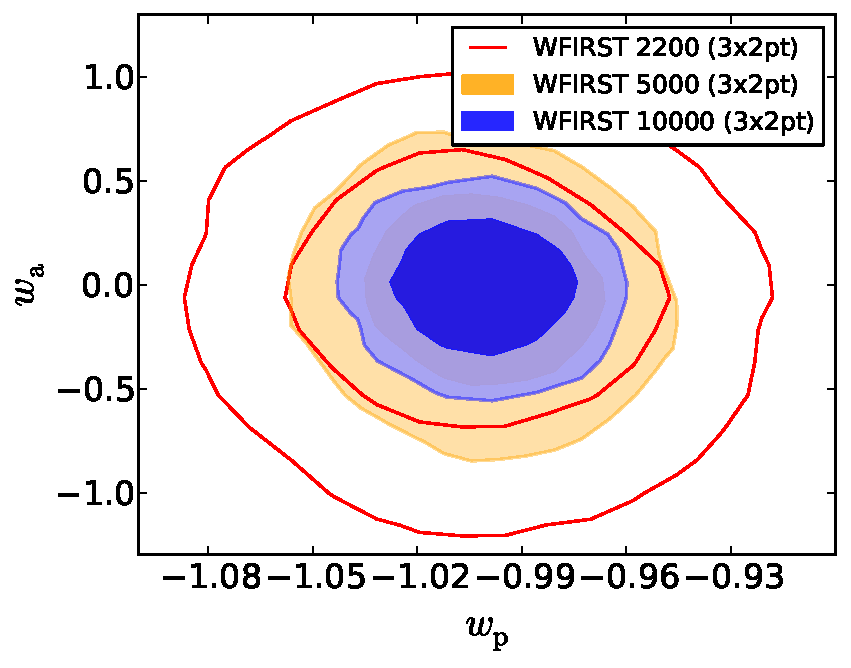
\includegraphics[width=8cm]{Plots/forecasts/WFIRST_extended.pdf}
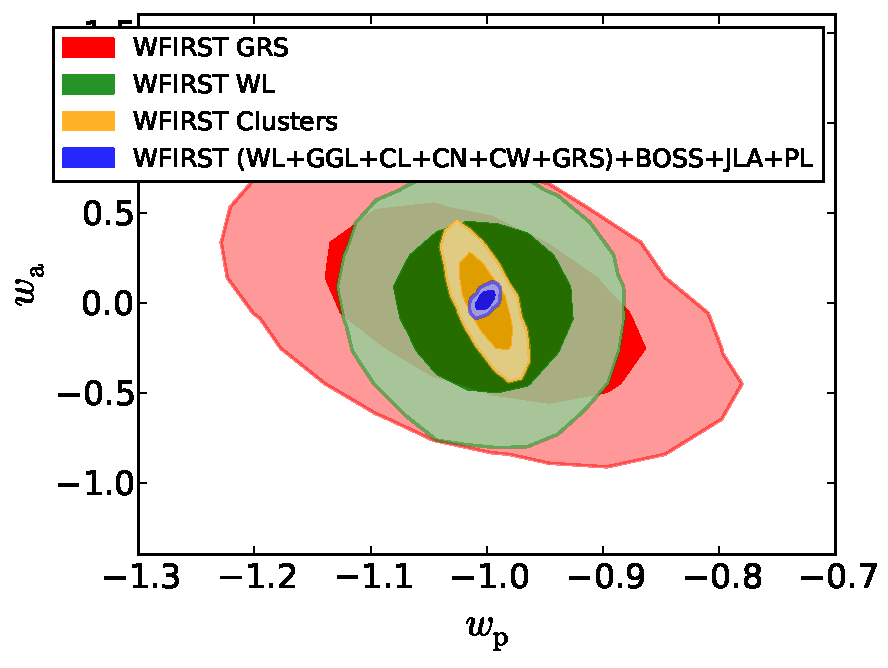
\includegraphics[width=8cm]{Plots/forecasts/WFIRST_ini_vs_multi.pdf}
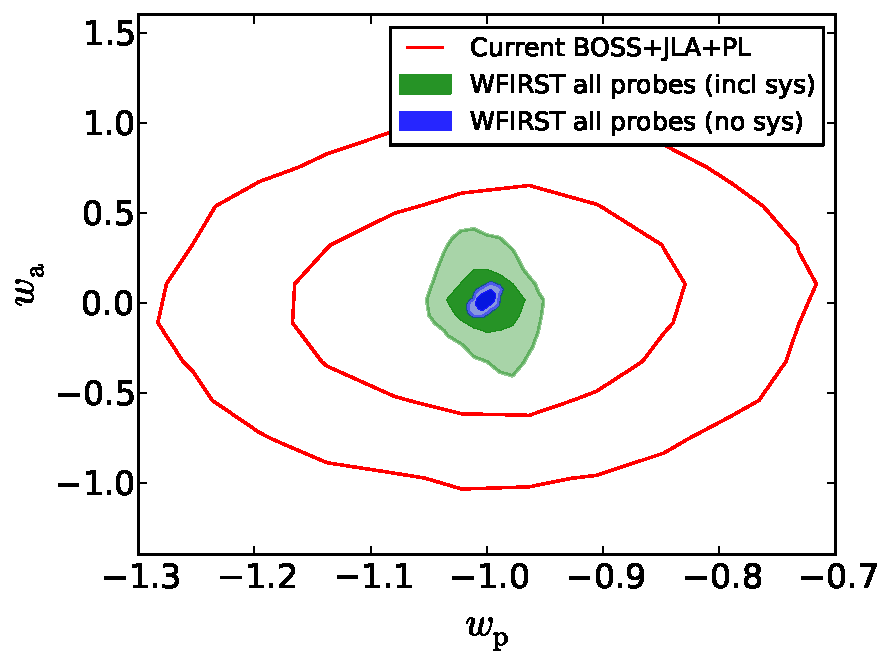
\includegraphics[width=8cm]{Plots/forecasts/WFIRST_multi_probe.pdf}
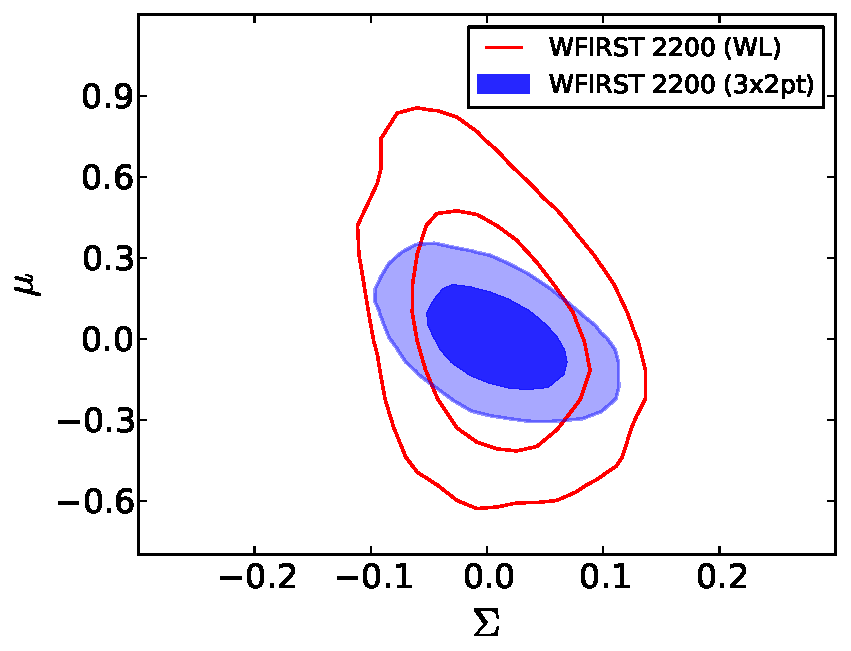
\includegraphics[width=8cm]{Plots/forecasts/WFIRST_shear_vs_MP.pdf}
\caption{LSST IA marg}
         \label{fi:lsst1}
\end{figure*}

Developing a multi-probe cosmology analysis framework is challenging given that the analysis pipeline for individual probes are each under continuous development in order to meet the requirements of improving data quality. These efforts have historically been largely independent from each other; as a consequence, individual probe analyses utilize information from other probes to offset/calibrate systematics. 
For example, one of the most important astrophysical uncertainties for galaxy clustering is the relation of dark matter halos and luminous galaxies. The joint analysis of clustering and galaxy-galaxy lensing measurements removes uncertainties in this halo-galaxy connection when constraining cosmology. However, cosmic shear analyses use the same galaxy-galaxy lensing measurements to offset other systematic uncertainties (e.g., intrinsic galaxy alignment). This is only one example of many systematics mitigation conflicts that can occur when considering probes in isolation.
A multi-probe analysis framework must account for these correlated systematic effects consistently across all probes; it cannot simply combine the optimal versions of individual analyses and it must include a global, well-designed systematics modeling and mitigation concept.
